\documentclass[10pt,a4paper]{article}
\usepackage{blindtext}
\usepackage{subcaption}
\usepackage{graphicx}
\usepackage{tikz}
\usepackage{amssymb}
\usepackage{caption}
\usepackage{amsmath}
\usepackage{circuitikz}
\usepackage{hyperref}
\usepackage{amssymb}
\usepackage{amsmath}
\usepackage{listings}

\lstset{
    inputencoding=utf8,
    extendedchars=true,
    literate={á}{{\'a}}1 {é}{{\'e}}1 {í}{{\'i}}1 {ó}{{\'o}}1 {ú}{{\'u}}1 {ñ}{{\~n}}1 {Á}{{\'A}}1 {É}{{\'E}}1 {Í}{{\'I}}1 {Ó}{{\'O}}1 {Ú}{{\'U}}1 {Ñ}{{\~N}}1
}
\usepackage[spanish,activeacute,es-tabla]{babel}
\usepackage[utf8]{inputenc}
\usepackage{ifthen}
\usepackage{listings}
\usepackage{dsfont}
\usepackage{subcaption}
\usepackage{amsmath}
\usepackage[strict]{changepage}
\usepackage[top=1cm,bottom=2cm,left=1cm,right=1cm]{geometry}%
\usepackage{color}%
\newcommand{\tocarEspacios}{%
	\addtolength{\leftskip}{3em}%
	\setlength{\parindent}{0em}%
}

% Especificacion de procs

\newcommand{\In}{\textsf{in }}
\newcommand{\Out}{\textsf{out }}
\newcommand{\Inout}{\textsf{inout }}

\newcommand{\encabezadoDeProc}[4]{%
	% Ponemos la palabrita problema en tt
	%  \noindent%
	{\normalfont\bfseries\ttfamily proc}%
	% Ponemos el nombre del problema
	\ %
	{\normalfont\ttfamily #2}%
	\
	% Ponemos los parametros
	(#3)%
	\ifthenelse{\equal{#4}{}}{}{%
		% Por ultimo, va el tipo del resultado
		\ : #4}
}

\newenvironment{proc}[4][res]{%
	
	% El parametro 1 (opcional) es el nombre del resultado
	% El parametro 2 es el nombre del problema
	% El parametro 3 son los parametros
	% El parametro 4 es el tipo del resultado
	% Preambulo del ambiente problema
	% Tenemos que definir los comandos requiere, asegura, modifica y aux
	\newcommand{\requiere}[2][]{%
		{\normalfont\bfseries\ttfamily requiere}%
		\ifthenelse{\equal{##1}{}}{}{\ {\normalfont\ttfamily ##1} :}\ %
		\{\ensuremath{##2}\}%
		{\normalfont\bfseries\,\par}%
	}
	\newcommand{\asegura}[2][]{%
		{\normalfont\bfseries\ttfamily asegura}%
		\ifthenelse{\equal{##1}{}}{}{\ {\normalfont\ttfamily ##1} :}\
		\{\ensuremath{##2}\}%
		{\normalfont\bfseries\,\par}%
	}
	\renewcommand{\aux}[4]{%
		{\normalfont\bfseries\ttfamily aux\ }%
		{\normalfont\ttfamily ##1}%
		\ifthenelse{\equal{##2}{}}{}{\ (##2)}\ : ##3\, = \ensuremath{##4}%
		{\normalfont\bfseries\,;\par}%
	}
	\renewcommand{\pred}[3]{%
		{\normalfont\bfseries\ttfamily pred }%
		{\normalfont\ttfamily ##1}%
		\ifthenelse{\equal{##2}{}}{}{\ (##2) }%
		\{%
		\begin{adjustwidth}{+5em}{}
			\ensuremath{##3}
		\end{adjustwidth}
		\}%
		{\normalfont\bfseries\,\par}%
	}
	
	\newcommand{\res}{#1}
	\vspace{1ex}
	\noindent
	\encabezadoDeProc{#1}{#2}{#3}{#4}
	% Abrimos la llave
	\par%
	\tocarEspacios
}
{
	% Cerramos la llave
	\vspace{1ex}
}

\newcommand{\aux}[4]{%
	{\normalfont\bfseries\ttfamily\noindent aux\ }%
	{\normalfont\ttfamily #1}%
	\ifthenelse{\equal{#2}{}}{}{\ (#2)}\ : #3\, = \ensuremath{#4}%
	{\normalfont\bfseries\,;\par}%
}

\newcommand{\pred}[3]{%
	{\normalfont\bfseries\ttfamily\noindent pred }%
	{\normalfont\ttfamily #1}%
	\ifthenelse{\equal{#2}{}}{}{\ (#2) }%
	\{%
	\begin{adjustwidth}{+2em}{}
		\ensuremath{#3}
	\end{adjustwidth}
	\}%
	{\normalfont\bfseries\,\par}%
}

% Tipos

\newcommand{\nat}{\ensuremath{\mathds{N}}}
\newcommand{\ent}{\ensuremath{\mathds{Z}}}
\newcommand{\float}{\ensuremath{\mathds{R}}}
\newcommand{\bool}{\ensuremath{\mathsf{Bool}}}
\newcommand{\cha}{\ensuremath{\mathsf{Char}}}
\newcommand{\str}{\ensuremath{\mathsf{String}}}

% Logica

\newcommand{\True}{\ensuremath{\mathrm{true}}}
\newcommand{\False}{\ensuremath{\mathrm{false}}}
\newcommand{\Then}{\ensuremath{\rightarrow}}
\newcommand{\Iff}{\ensuremath{\leftrightarrow}}
\newcommand{\implica}{\ensuremath{\longrightarrow}}
\newcommand{\IfThenElse}[3]{\ensuremath{\mathsf{if}\ #1\ \mathsf{then}\ #2\ \mathsf{else}\ #3\ \mathsf{fi}}}
\newcommand{\yLuego}{\land _L}
\newcommand{\oLuego}{\lor _L}
\newcommand{\implicaLuego}{\implica _L}

\newcommand{\cuantificador}[5]{%
	\ensuremath{(#2 #3: #4)\ (%
		\ifthenelse{\equal{#1}{unalinea}}{
			#5
		}{
			$ % exiting math mode
			\begin{adjustwidth}{+2em}{}
				$#5$%
			\end{adjustwidth}%
			$ % entering math mode
		}
		)}
}

\newcommand{\existe}[4][]{%
	\cuantificador{#1}{\exists}{#2}{#3}{#4}
}
\newcommand{\paraTodo}[4][]{%
	\cuantificador{#1}{\forall}{#2}{#3}{#4}
}

%listas

\newcommand{\TLista}[1]{\ensuremath{seq \langle #1\rangle}}
\newcommand{\lvacia}{\ensuremath{[\ ]}}
\newcommand{\lv}{\ensuremath{[\ ]}}
\newcommand{\longitud}[1]{\ensuremath{|#1|}}
\newcommand{\cons}[1]{\ensuremath{\mathsf{addFirst}}(#1)}
\newcommand{\indice}[1]{\ensuremath{\mathsf{indice}}(#1)}
\newcommand{\conc}[1]{\ensuremath{\mathsf{concat}}(#1)}
\newcommand{\cab}[1]{\ensuremath{\mathsf{head}}(#1)}
\newcommand{\cola}[1]{\ensuremath{\mathsf{tail}}(#1)}
\newcommand{\sub}[1]{\ensuremath{\mathsf{subseq}}(#1)}
\newcommand{\en}[1]{\ensuremath{\mathsf{en}}(#1)}
\newcommand{\cuenta}[2]{\mathsf{cuenta}\ensuremath{(#1, #2)}}
\newcommand{\suma}[1]{\mathsf{suma}(#1)}
\newcommand{\twodots}{\ensuremath{\mathrm{..}}}
\newcommand{\masmas}{\ensuremath{++}}
\newcommand{\matriz}[1]{\TLista{\TLista{#1}}}
\newcommand{\seqchar}{\TLista{\cha}}

\renewcommand{\lstlistingname}{Código}
\lstset{% general command to set parameter(s)
	language=Java,
	morekeywords={endif, endwhile, skip},
	basewidth={0.47em,0.40em},
	columns=fixed, fontadjust, resetmargins, xrightmargin=5pt, xleftmargin=15pt,
	flexiblecolumns=false, tabsize=4, breaklines, breakatwhitespace=false, extendedchars=true,
	numbers=left, numberstyle=\tiny, stepnumber=1, numbersep=9pt,
	frame=l, framesep=3pt,
	captionpos=b,
}

\newcommand{\notimplies}{\;\not\!\!\!\implies}
\title{Algoritmos y Estructuras de Datos II}
\author{Tomás Agustín Hernández}
\date{}

\begin{document}
\maketitle

\begin{figure}[b]
    \centering
    \begin{tikzpicture}[remember picture,overlay]
        \node[anchor=south east, inner sep=0pt, xshift=-1cm, yshift=2cm] at (current page.south east) {
            \begin{minipage}[b]{0.5\textwidth}
                
\includegraphics[width=\linewidth]{logo_uba.jpg}
                \label{fig:bottom}
            \end{minipage}
        };
    \end{tikzpicture}
\end{figure}

\newpage
\section{Especificación}
\subsection*{Consideraciones importantes / Reminders}
\begin{itemize}
    \item Utilizar operadores luego: Si estoy en LPO (Lógica de Primer Orden) utilizar los operadores luego si vemos que hay una posible indefinición como una división, o ingresar a una lista a un índice. Recordar que el para todo y un existe, aunque esté acotado por un rango, los cuantificadores predican IGUAL para todos los valores. Entonces, aunque diga que x es positivo, también probará dividir inclusive por 0 y estallará.
    \item Recordar las condiciones bidireccionales
        \begin{itemize}
            \item Si por algún motivo tengo que armar una “lista”, como, por ejemplo, los divisores de un número x tengo que indicar que, si el número divide a x, entonces ese número está en res, pero además todos los valores que están en res DIVIDEN a x. Es una condición bidireccional. 
            \item Otro ejemplo puede ser que tenga que considerar el máximo de una lista, si todos los valores y que están en la lista son menores que res entonces significa que res también pertenece a esa lista original.
        \end{itemize}
    \item Recordar el significado de los cuantificadores con dos variables al mismo tiempo: En la lógica se ejecutan todos de uno a la vez. Es decir, si tengo que poner un para todo adentro de un para todo entonces hago un para todo solo con dos variables y listo.
    \item Recordar que cuando en un procedimiento llamo a un predicado y ese predicado devuelve algo de un para todo, existe (básicamente un valor de verdad) tengo que castear ese valor en el procedimiento porque son dos mundos distintos.
    Ej: asegura: { res = True \(\iff\) predicado}
    \item Los predicados y funciones auxiliares no describen problemas. Son herramientas sintácticas para descomponer predicados.
    \begin{itemize}
        \item Los procedimientos pueden llamar a funciones auxiliares o predicados. Un procedimiento no puede llamar a otro procedimiento.
        \item Los predicados pueden llamar a predicados o auxiliares. 
        \item Las auxiliares solo pueden llamar auxiliares.
    \end{itemize}
    \item No usamos nunca \(==\) en especificación, usamos siempre \(=\) y estamos comparando, no asignando.
    \item No existe el guardar o asignar en el mundo de la lógica. No puedo guardar en una lista en un índice específico porque si un valor. Para esto solemos usar que x valor pertenecerá a esta lista, por ejemplo.
    \item Si tengo un algoritmo que cumple una funcionalidad específica con un require más débil, puedo poner el require más restrictivo y va a funcionar igual pero NO al revés.
\end{itemize}
\subsection*{Fórmulas compuestas}
Decimos que una fórmula es compuesta a una fórmula que tiene más de una operación y esa operación necesita realizarse antes de conocer su valor.
\begin{itemize}
    \item \((p \land q) \lor m\)
    \item \(((p \land q) \lor m) \implies n\)
\end{itemize}
\subsection*{Fórmula atómica}
Decimos que una fórmula es atómica si se puede inferir su valor con una, o ninguna operación. Es irreducible.
\begin{itemize}
    \item p
    \item \(p \land q\)
\end{itemize}
\subsection*{Fórmulas bien definidas}
Decimos que una fórmula está bien definida cuando el orden que hay que hacer las operaciones es clara. Es decir, cuando cada operación toma dos variables proposicionales, y al realizar la operación termina siendo una fórmula atómica.
\begin{itemize}
    \item \(p \land q \lor r\) está mal formada. No se especifica si primero se realiza el \(\land\) o el \(\lor\).
    \item \((p \land q) \lor r\) está bien formada.
    \item \(p \land q \land r \land m\) está bien formada porque son todas conjunciones.
    \item \(p \lor q \lor r \lor m\) está bien formada porque son todas disyunciones.
\end{itemize}
\subsection*{Cuantificadores}
\begin{itemize}
    \item Para todo: \(\forall\)
    \begin{itemize}
        \item \(Garantiza \ la \ \text{conjunción}: p(1) \land p(2) \land p(3) \dots \land p(m) \). Todos los casos deben ser \True \ para que el cuantificador sea \True.
        \item Se acompaña por un \(\implica\) a la hora de predicar sobre los elementos.
        \item \((\forall i: \ent)(0 \le i < \longitud{s} \implicaLuego \ s[i] \ mod \ 2 = 0)\). Todos los elementos de la lista son divisibles por 2.
        \item Estructura: \(\forall\) + rango + \(\implicaLuego\)
    \end{itemize}
    \item Existe: \(\exists\)
    \begin{itemize}
        \item \(Garantiza \ la \ \text{disyunción}: p(1) \lor p(2) \lor p(3) \dots \lor p(m) \). Con un caso \True \ el cuantificador es \True.
        \item Se acompaña por un \(\land\) a la hora de predicar sobre los elementos.
        \item \((\exists i: \ent)(0 \le i < \longitud{s} \yLuego s[i] \ge 0)\). Existe algún elemento en la lista que es mayor o igual a 0.
        \item \(\exists\) + rango + \(\yLuego\)
    \end{itemize}
\end{itemize}
\subsection*{Equivalencias entre fórmulas}
Decimos que dos fórmulas son equivalentes \(\iff\) los valores de la tabla de verdad al aplicar la operación arroja el mismo resultado.

\subsection*{Valuaciones}
Las valuaciones surgen en base a la tabla de verdad. Las valuaciones serian darle valor a las variables proposicionales y ver el resultado de la operación. Solo hacen referencias a fórmulas atómicas.

\subsection*{Tautologias, contradicciones y contingencias}
\begin{itemize}
    \item Una fórmula es tautología \(\iff\) el resultado de la operación en cada fila arroja siempre V.
    \item Una fórmula es contradicción \(\iff\) el resultado de la operación en cada fila arroja siempre F.
    \item  Una fórmula es contradicción \(\iff\) el resultado de la operación en cada fila arroja siempre V y F.
\end{itemize}

\subsection*{Relaciones de fuerza entre fórmulas}
Decimos que una fórmula es más fuerte que la otra \(\iff\) una fórmula es más restrictiva que la otra, o está incluida en la otra. \\
En el mundo de la lógica, decimos que A es más fuerte que B \(\iff A \implies B\)

\begin{itemize}
    \item Si (\(A \implies B\)) y (\(B \implies A\)) son tautologías, entonces A y B son equivalentes.
    \item Si (\(A \implies B\)) es tautología y (\(B \notimplies A\)) no es tautología, entonces decimos que A es más fuerte que B.
    \item Si (\(A \notimplies B\)) y (\(B \notimplies A\)) son contigencias, entonces no existe relación de fuerza entre A y B.
\end{itemize}

Algunos ejemplos:

\begin{itemize}
    \item \(\longitud{s} = 0 \implies \longitud{s} \ge 0\). En este caso vemos que \(\longitud{s} = 0\) es más fuerte que \(\longitud{s} \ge 0\) pues \(\longitud{s} = 0\) está incluido en \(\longitud{s} \ge 0\). Por lo tanto, \(A \implies B\)
    \item \(\longitud{s} = 0 \implies \longitud{s} \ge 3\). En este caso vemos que \(\longitud{s} = 0\) no es más fuerte que \(\longitud{s} \ge 3\) pues \(\longitud{s} = 0\) no está incluido en \(\longitud{s} \ge 3\). Por lo tanto, \(A \notimplies B\)
    \item \(2 \le i < \longitud{s} \implies 1 \le i < \longitud{s}\). En este caso A \(\implies\) B, pues i = 2 está incluido en el rango de B. Por lo tanto, \(A \implies B\)
    \item \(0 \le i < \longitud{s} \implies 1 \le i < \longitud{s}\). En este caso A \(\notimplies\) B, pues el 0 de A no es parte de B. Por lo tanto, \(A \notimplies B\)
\end{itemize}

\subsection*{Tipos de parámetros en especificacion}
\begin{itemize}
    \item in: Solo nos interesa el valor de entrada de una variable. No la vamos a modificar. Ya están inicializados
    \item out: Donde se retornará el resultado. No nos importa el valor inicial ni tampoco determina nada en nuestra función.
    \item inout: Necesitamos el valor original aunque lo terminamos modificando y devolviendo.
\end{itemize}
\subsection*{Lógica trivaluada}
También llamada lógica secuencial porque se procesa de izquierda a derecha; Nos introduce los conceptos de \(\yLuego \ \oLuego \ \implicaLuego\) y el valor de indefinido \(\bot\).

Se termina de evaluar una expresión cuando se puede deducir el valor de verdad. \\


Considere \(x = \True \land y = \bot \land z = \False \)
\begin{itemize}
    \item \(x \oLuego y\): Como el \(\oLuego\) necesita uno solo para ser verdadero, entonces como x ya es \(\True\) entonces toda la fórmula es verdadera.
    \item \(x \yLuego y\): Como el \(\yLuego\) necesita que ambas variables sean verdaderas, evalúa indefinido y el programa estalla.
    \item \(\neg x \implicaLuego y\): Como el \(\implicaLuego\) solo es falso si el antecedente es  \(\True\) y el consecuente \(\False\), como en este caso el antecedente ya es falso, toda la implicación es verdadera.
    \item \((x \land z) \yLuego y\): Como el \(\yLuego\) necesita que ambas fórmulas sean \(\True\), en este caso, como \((x \land z)\) es falso, entonces ya toda la fórmula es falsa. Nótese que el \(\land\) de la condición interna no contiene el luego porque jamás se indefinirá.
    \item \((\forall i: \ent)(0 \le i < \longitud{s} \implicaLuego s[i] \ge 0)\) Nótese que aquí usamos un \(\implicaLuego\) porque podría ser que la lista esté indefinida o no exista el valor en s[i]
\end{itemize}

\subsection*{Predicados}
\begin{itemize}
    \item Viven en el mundo de la lógica. 
    \item Nos sirven para poder modularizar nuestras especificaciones. 
    \item Solamente devuelven valores de verdad True y False y es necesario castearlos en caso de querer devolver bool como tipo de dato.
    \item Los predicados pueden llamar a otros predicados o funciones auxiliares.
    \item Pueden utilizar cuantificadores.
    \item No tienen requiere ni asegura.
    \item No admite parámetros in, out, inout.
\end{itemize}

\leavevmode
\\
Ejemplo cuando tenemos que transformar el valor de verdad a tipo de dato: 
\leavevmode
\\
\pred{divisiblePorDos}{n: \ent}{
    n \ mod \ 2 = 0
}

\begin{proc}{esMultiploDeDos}{\In n: \ent}{\bool}
    \requiere{\True}
    \asegura{res = true \iff divisiblePorDos(n)}
\end{proc}
\leavevmode
\\ 
Ejemplo usando un predicado sin necesidad de transformar el valor de verdad a tipo de dato: 

\leavevmode
\pred{todosSonPares}{l: \TLista{\ent}}{
    \paraTodo[unalinea]{i}{\ent}{0 \le i < \longitud{l}  \implicaLuego l[i] mod 2 = 0}
}

\begin{proc}{todosPares}{\In l: \TLista{\ent}}{\bool}
    \requiere{todosSonPares(l)}
\end{proc}
\newpage
\subsection*{Funciones Auxiliares}
\begin{itemize}
    \item Son reemplazos sintácticos. 
    \item Nos ayudan a modularizar las especificaciones.
    \item No pueden ser recursivas.
    \item Solo hacen cuentas.
    \item No pueden utilizar cuantificadores.
    \item Pueden llamar a predicados.
    \item Devuelven un tipo de dato.
    \item No tienen requiere ni asegura.
    \item No admite parámetros in, out, inout.
\end{itemize}

\leavevmode
\aux{sumar}{n: \ent, m: \ent}{\ent}{
    n + m
}

\aux{sumarTodos}{s: \TLista{\ent}}{\ent}{
    \sum_{i=0}^{\longitud{s}-1}{s[i]}
}


\subsection*{Aridad}
Decimos que una función es de aridad \(n\) cuando la función recibe \(n\) cantidad de parámetros.

\subsection*{Variables Ligadas y Libres}
Las variables son ligadas \(\iff\) están dentro de un cuantificador mientras que son libres cuando no lo están.
\begin{itemize}
    \item \((\forall i: \ent)(0 \le i < \longitud{s} \implicaLuego n \ge s[i])\) i es una variable ligada mientras que n y s son variables libres.
    \item \((\exists j: \ent)(0 \le j < \longitud{s} \yLuego n \ge s[i])\) j es una variable ligada mientras que n y s son variables libres.
    \item \((\forall i: \ent)(0 \le i < \longitud{s} \implicaLuego n \ge s[i]) \land P(i)\) Ojo acá. i es una variable ligada, pero la i que está fuera del cuantificador \(P(i)\) no está ligada. Esta última debería ser renombrada para no tener problemas y confusiones.
\end{itemize}

Cuando tenemos variables ligadas \textbf{no} podemos hacer nada sobre ellas, entre esas cosas, no podemos reemplazarlas porque no dependen de nosotros sino de los cuantificadores.

\subsection*{Cuantificadores anidados}
Anidamos cuantificadores cuando el rango de las variables es exactamente el mismo.
\begin{itemize}
    \item \((\forall i, j: \ent)(0 \le i, j < \longitud{s} \implicaLuego n \ge s[i][j]) \equiv (\forall i: \ent)((0 \le i < \longitud{s}\implicaLuego (\forall  j: \ent)(0 \le j < \longitud{s} \implicaLuego n \ge s[i][j]))) \) 
\end{itemize}

\subsection*{Estado}
Llamamos estado a los valores de las variables en un punto de ejecución específico. El estado de un programa es importante porque muta al asignar valores a las variables.
Cuando necesitamos hablar del estado de una variable en un instante específico, hablamos de \textbf{metavariables} \\ 

\subsection*{Metavariables}
Llamamos metavariable a una variable en un instante dado. Es útil cuando tenemos que predicar como cambio el valor de una variable con respecto al inicial. \\
Cuando tenemos que utilizar metavariables, sea S una variable cualquiera podemos referirnos al instante de tiempo de S como \(S_{t}\) donde t indica el momento. \\ \\ 
Notación \(S = S_{0}\)

\begin{proc}{multiplicarPorDosAImpares}{\Inout l: \TLista{\ent}}{}
    \requiere{l = l_{0}}
    \asegura{\longitud{l} = \longitud{l_{0}}}
    \asegura{(\forall i: \ent)(0 \le i < \longitud{s} \implicaLuego if(s_{0} [i] \ mod \ 2 \neq 0) \ then \ (s[i] = s_{0}[i] \ast 2) \ else \ (s[i] = s_{0}[i]) \ fi)}
\end{proc}
\leavevmode
\\
Nota: Cuando utilizamos metavariables tenemos que indicar que al modificar algo directamente, si no modificamos todo el conjunto de valores tenemos que indicar que los demás permanecen inalterados. En este caso, como estamos editando los valores, no tendría sentido que la lista salga con mayor longitud, es por eso que garantizamos que no cambia. 

Otra manera de resolver el ejemplo anterior es utilizando old(s)
\begin{proc}{multiplicarPorDosAImpares}{\Inout l: \TLista{\ent}}{}
    \asegura{\longitud{l} = \longitud{old(l)}}
    \asegura{(\forall i: \ent)(0 \le i < \longitud{s} \implicaLuego if(old(s)[i] \ mod \ 2 \neq 0) \ then \ (s[i] = old(s)[i] \ast 2) \ else \ (s[i] = old(s)[i]) \ fi)}
\end{proc}
\leavevmode
\\

\section*{Correctitud de un Programa}
Decimos que un programa S es correcto respecto a una especificación si se cumple la precondición P, el programa termina su ejecución y se cumple la postcondición Q.
\subsection*{Tripla de Hoare}
Notación para indicar que S es correcto respecto a la especificación (P, Q) \\ 
\[\{P\} \ S \ \{Q\}\]

\subsection*{SmallLang}
Es un lenguaje que nos permitirá poder validar la correctitud de un programa.
Solo tiene dos operaciones: 
\begin{itemize}
    \item x := E \(\equiv\) asignación
    \item skip \(\equiv\) no hace nada
\end{itemize}

Nota: E es una expresión cualquiera. Un valor, una función, cualquier cosa.

\subsection*{Estructuras de Control en SmallLang}
\begin{itemize}
    \item Secuencia de pasos: S1; S2 es un programa \(\iff\) S1 y S2 son dos programas.
    \item Condicionales: if B then S1 else S2 endif es un programa \(\iff\) B es una condición lógica (guarda) y S1 y S2 son programas.
    \item Ciclo: while B do S endwhile es un programa \(\iff\) B es una condición lógica y S un programa.
\end{itemize}

\subsection*{Validez de una tripla de Hoare}
\(\{x \ge 4\} \ x := x+1 \ \{x \ge 7\}\)
Donde, 
\begin{itemize}
    \item P = \(\{x \ge 4\}\)
    \item S = \(x := x+1\)
    \item Q = \(\{x \ge 7\}\)
\end{itemize}

¿Vale que \(\{P\} \ S \ \{Q\}\)?
Solo vale \(\iff x \ge 6\) por lo tanto, como la precondición P falla en los casos de x = 4, x = 5 podemos decir que la tripla de Hoare no es válida.\\

Esto que acabamos de hacer se llama demostrar la correctitud de un programa, y acabamos de demostrar que la precondición P para el programa S es demasiado débil pues no nos garantiza que llegaremos a Q cumpliendo P. \\

Existe una manera formal que nos permite conocer la precondición más débil de un algoritmo.
\newpage
\subsection*{Predicado def(E)}
Dada una expresión E, llamamos def(E) a las condiciones para que E esté definida. Todas las constantes están definidas, por lo tanto def(x) \(\equiv\) True. La idea es ir separando en términos e ir colocando las definiciones necesarias para esa operación específica.
\begin{itemize}
    \item \(def(x+1) \equiv def(x) \land def(1) \equiv True \land True \equiv True\)
    \item \(def(x/y) \equiv def(x) \land (def(y) \land y\neq0) \equiv True \land (True \land y>0) \equiv y\neq0\)
    \item \(def(\sqrt{x}) \equiv (def(x) \land x\ge0)\)
    \item \(def(a[i]+3) \equiv (def(a) \land def(i)) \yLuego 0 \le i<\longitud{a} \land def(3) \equiv (True \land True) \yLuego 0\le i<\longitud{a} \land True \equiv 0\le i<\longitud{a}\)
\end{itemize}

\subsection*{Predicado \(Q^{x}_{E}\)}
Cuando hablamos de este predicado hablamos de reemplazar las ocurrencias de x por E en el programa. Solo se reemplazan las ocurrencias libres, no las ligadas.
\subsection*{Axiomas}
\begin{itemize}
    \item Axioma 1: \(wp(x := E, Q) \equiv def(E) \yLuego Q^{x}_{E}\)
    \item Axioma 2: \(wp(skip, Q) \equiv Q\)
    \item Axioma 3: \(wp(S1; S2, Q) \equiv wp(S_{1}, wp(S_{2}, Q))\)
    \item Axioma 4: \(wp(S, Q) \equiv def(B) \yLuego ((B \land wp(S_{1}, Q)) \lor (\neg B \land wp(S_{2}, Q)))\)
\end{itemize} 

\subsection*{Axioma 1 con secuencias}
El axioma 1 nos sirve para asignar una expresión a una variable; Sin embargo, si tenemos que guardar algo en una secuencia debemos utilizar el setAt.
\begin{itemize}
    \item \(wp(b[i]:=E, Q) \\
    \equiv def(setAt(b, i, E)) \yLuego Q^{b[i]}_{setAt(b, i, E)} \\
    \equiv (def(b) \land def(i) \land def(E)) \yLuego 0\le i < \longitud{b} \yLuego Q^{b[i]}_{setAt(b, i, E)} \\
    \equiv 0\le i < \longitud{b} \yLuego Q^{b[i]}_{setAt(b, i, E)}   \\
    \equiv setAt(b, i, E)[j] = \{E \ si \ i = j, b[j] \ si \ i \neq j\}\)
\end{itemize}

Algunos ejemplos:\\
\(wp(s[i]:=s[i-1], Q) \\
wp(setAt(s, i, s[i-1]), Q) \equiv \\
def(setAt(s, i, s[i-1])) \equiv (def(s) \land def(i)) \yLuego 0 \le i < \longitud{s} \yLuego def(s[i-1]) \equiv \\ 0\le i < \longitud{s} \yLuego (def(s) \land def(i)) \yLuego 0\le i-1 < \longitud{s} \equiv  0\le i < \longitud{s} \yLuego 1\le i < \longitud{s} + 1 \equiv  \textcolor{blue}{1 \le i < \longitud{s}}
\)


TODO: Luego mostrar un ejercicio y aclarar que por cada condición se separan n cuantificadores.

\subsection*{Precondición más débil (Weakest Precondition)}
Es la precondición más débil que se necesita para poder ejecutar un algoritmo y satisfacer la postcondición Q. \\ \\
Notación: \(wp(S, Q)\) donde S es el programa y Q la postcondición. \\ \\
Teorema: Una tripla de Hoare \(\{P\} \ S \ \{Q\}\) es válida \(\iff P \implicaLuego wp(S, Q)\). \\ \\ 
Sea el siguiente enunciado, calcule la precondición más debil.
\begin{itemize}
    \item P = \(\{x \ge 4\}\)
    \item S = \(x := x+1\)
    \item Q = \(\{x \ge 5\}\)
\end{itemize} 
\(P \implicaLuego wp(S, Q) \equiv wp(x := x+1, x \ge 5) \equiv def(x+1) \yLuego Q^{x}_{x+1} \equiv def(x) \yLuego def(1) \yLuego x+1 \ge 5 \\ \equiv True \yLuego True \yLuego x \ge 4 \equiv x \ge 4\)

Luego, \(\{x \ge 4\} \implicaLuego \{x \ge 4\}\) es \(\True\)

Por lo tanto, \(wp(x:=x+1, x \ge 5) \equiv \{x \ge 4\}\)

Finalmente, probamos que para poder satisfacer Q la precondición más debil que cumple P es cuaqluier \(x \ge 4\). \\

Nota importante: Muchas veces puede ser que se nos solicite indicar que \(wp\) es incorrecta. Cuando se dice esto, significa que son precondiciones válidas pero hay algunas que no son la más débil.

\newpage 
\section*{Precondición más débil en ciclos}
Consideremos el siguiente ejemplo
\(\{???\} S \{x=0\}\)
donde S es el siguiente programa 

\begin{lstlisting}
     while(x>0) do
        x := x-1
    endwhile
 \end{lstlisting}

 Recordemos que esto es una tripla de Hoare, pero no podemos utilizar wp(S, Q) porque el programa es en base a ciclos. La precondición P más débil acá sería que x\(\ge\)0 porque para cumplir la postcondición Q me da igual si entra al ciclo o no.
 Eso tiene que quedar siempre claro, cuando estamos hablando en ciclos, si no entra al ciclo y satisface igual ya está.
 \subsection*{Predicado \(H_{k}\)}
 Definimos el predicado \(H_{k}\) para poder controlar la cantidad de iteraciones que hace un ciclo y poder calcular la precondición más débil.
 \begin{itemize}
    \item \(H_{0}(Q) \equiv def(B) \land \neg B \land Q\)
    \item \(H_{k+1}(Q) \equiv def(B) \land B \land wp(S, H_{k}(Q)) \ para \ k \ge 0\) 
\end{itemize} 
\subsection*{Axiomas}
Definimos el Axioma 5 para poder verificar la correctitud de ciclos que hacen una cantidad de iteraciones fijas como \\
\[wp(while \ B \ do \ S \ endwhile, Q) \equiv (\exists_{i\ge0})(H_{i}(Q))\]

¿Cual es el problema del Axioma 5 y el Predicado \(H_{k}\)? El problema es que ambos nos sirven para poder validar la precondición de un ciclo que sabemos que finaliza luego de \(n\) iteraciones.

\subsection*{Predicado \(I\) - Invariante}
Definimos el Invariante de un ciclo como un predicado que:
\begin{itemize}
    \item Demuestra que el ciclo realmente funciona y nos ayuda a demostrar la correctitud parcial "si termina el ciclo... entonces se cumple Q"
    \item Vale antes de entrar al ciclo y luego de salir del ciclo.
    \item En cada iteración, el invariante debe volver a ser válido. En el medio de la iteración puede que deje de valer.
    \item Un buen invariante incluye el rango de la(s) variable(s) de control del ciclo.
    \item Un buen invariante tiene alguna afirmación sobre el acumulador del ciclo.
\end{itemize} 

\subsection*{Teorema del Invariante}
Para poder probar que un ciclo es correcto, usamos el teorema del invariante.
\begin{itemize}
    \item \(P \equiv \) Las condiciones del requiere
    \item \(P_{c} \equiv\) Las precondiciones que necesita el ciclo para poder ingresar, muchas veces son las líneas que están por encima del while y el requiere (¡no todas las del requiere!)
    \item \(I \equiv \) Las condiciones que suceden antes y después de entrar al ciclo
    \item \(B \equiv \) La guarda del ciclo
    \item \(Q_{c} \equiv\) La postcondición del ciclo
  
\end{itemize} 
Luego, 
\begin{itemize}
    \item \(\ \{P\} \ S \ \{P_{c}\}\)
    \item \(\ P_{c} \implies I\)
    \item \(\{I \land B\} \ S \ \{I\}\)
    \item \(\{I \land \neg B\} \implies Q_{c}\)
\end{itemize} 
\textbf{Recordatorio}: Si aparece la S es que tenemos que calcular la wp porque es parte de la Tripla de Hoare. \\
\textbf{Recordatorio importante}: Para todo lo que es wp usamos SmallLang, es decir, cuando tenemos que validar la tripla de Hoare. En todos los demás casos usamos lógica. \\
Ej: No sería válido tener un if en un invariante.
\subsection*{Teorema de Terminación de Ciclo}
Utilizamos el teorema de terminación de ciclo para garantizar que cumpliendo la precondición de un ciclo, el programa siempre termina.
Para poder probar esto, necesito una función variante \(f_{v}\). \\
Llamamos función variante \(f_{v}\) a una función que es siempre estrictamente decreciente y representa una cantidad que se va reduciendo a lo largo de las iteraciones.
La función \(f_{v}\) debe garantizar
\begin{itemize}
    \item \(\{I \land B \land v_{0} = f_{v}\} \ S \ \{f_{v} < v_{0}\}\)
    \item \(\{I  \land f_{v} \le 0 \implies \neg B\}\)
   
\end{itemize}
\subsection*{Reglas generales para validar correctitud de ciclo y terminación}
\begin{itemize}
    \item Cuando tenemos que iterar sobre listas, tendremos un índice i que irá hasta incluida la longitud (pues nos sirve) para negar la guarda, mientras que el j será para usar dentro del ciclo. 
    \((0\le i \le \longitud{s} \yLuego (0 \le j < i \implicaLuego res = \sum_{j=0}^{i}{s[j]}))\)
    \item Si tengo algo en \(I\) deberá estar en \(P_{c}\) y/o \(Q_{c}\). Esto es porque cuando tengamos que hacer las implicancias, deberíamos comparar de ambos lados y si el invariante tiene algo que los demás no, es siempre falso. 
    \item Si tengo algo en \(P_{c}\) o \(Q_{c}\) no necesariamente tiene que estar en \(I\)
    \item En \(Q_{c}\) se acostumbra a colocar que \(i = \longitud{s}\) porque nos ayuda a demostrar la terminación del ciclo.
    \item En la función variante: i va negada si i crece en el ciclo; i va positivo si i decrece en el ciclo.
    \item En \(Q_{c}\) rara vez tenemos que hablar de rangos de variables.
\end{itemize} 

\section*{TADs (Tipos Abstractos de Datos)}
Es un tipo de datos porque define un conjunto de valores y las operaciones que se pueden realizar sobre ellos. Es abstracto ya que para utilizarlos no necesitamos saber como está implementado.
Describe el qué y no el cómo.
Son una forma de modularizar a nivel de los datos.  \\ \\
Importante: En todo enunciado ambiguo, queda en nosotros interpretarlo y eliminar esas ambiguedades decidiendo como lo vamos a considerar.\\ \\
Ej: En varios ejercicios te piden que un punto deba cambiarse el centro y hay dos maneras de plantearlo
\begin{itemize}
    \item Agarrar el centro que vienen por parámetro y sumar coordenada a coordenada con respecto a las de la instancia de mi TAD. 
    \item Agarrar el centro que viene por parámetro y considerarlo como el centro final en la instancia del TAD.
\end{itemize}
Importante: En un TAD podemos usar todos los mismos tipos de datos de especificación y sus funciones correspondientes.

\subsection*{Observadores}
Los observadores son una especie de atributo en un objeto en POO.
Nos permiten saber qué valores tienen y en qué momento.
\begin{itemize}
    \item Sirven para describir el estado de una instancia de un TAD y nos permiten consultar su estado virtual.
    \item Tenemos que poder observar todas las características que nos interesan de las instancias.
    \item En un instante de tiempo, el estado de una instancia del TAD estará dado por el estado de todos sus observadores (como un debugger).
    \item Nos permiten distinguir si dos instancias son distintas.
    \item Todas las operaciones tienen que poder ser descriptas a partir de los observadores.
\end{itemize} 
Ejemplo de un TAD con observadores de tipo dato:
\begin{lstlisting}
    TAD lista {
        obs elems: conj<T>
        obs cantElems: int
    }
\end{lstlisting}

Los observadores también pueden ser funciones auxiliares.
\begin{itemize}
    \item Son las auxiliares de nuestro lenguaje de especificación 
    \item No pueden tener efectos colaterales ni modificar los parámetros
    \item Pueden usar tipos de nuestro lenguaje de especificación 
\end{itemize} 
Ejemplo de un TAD con observadores de tipo dato:
\begin{lstlisting}
    TAD lista {
        obs elems: conj<T>
        obs estaElem(e: T): bool
    }
\end{lstlisting}

\subsection*{Igualdad Observacional}
Decimos que dos TADs son iguales \(\iff\) todos sus observadores son iguales.\\
Muchas veces no nos basta con la igualdad por defecto con los observadores, y tenemos que declarar nuestra propia igualdad observacional.

\subsection*{Operaciones de un TAD}
Las operaciones de un TAD deben estar especificadas y nos indican qué se puede hacer con una instancia.
Antes y una vez aplicada una operación tenemos que hablar del estado en el que quedó el TAD con respecto a sus observadores.
\section*{Implementación de un TAD}
\subsection*{Módulos}
\begin{itemize}
    \item Son la representación / implementación física en código de un TAD.
    \item Los módulos implementan el TAD.
    \item Un procedimiento de un módulo puede llamar a otros procedimientos del módulo.
\end{itemize}
\subsection*{Variables de Estado}
Lo que en los TADs eran observadores, acá son variables de estado. Serán manipuladas por las operaciones mediante el código de los algoritmos. 
Tipos válidos para variables de estado: 
\begin{itemize}
    \item int, real, bool, char, string
    \item tupla\(<\)T1, T2, T3\(>\), struct\(<\)campo1: val1, campo2: val2\(>\)
    \item Array\(<\)T\(>\) (arrays de tamaño fijo)
    \item No es posible usar tipos de especificación como conj\(<\)T\(>\) o seq\(<\)T\(>\)
\end{itemize}
El módulo puede tener variables de estado que no hagan referencia a ningún observador de un TAD, por ejemplo: guardar un máximo en un módulo aunque el TAD no lo pida. A veces estas cosas se hacen solo por temas de a la hora de implementarlo en un lenguaje de programación. \\ 
\textbf{Nota: Una variable de estado también puede contener otro módulo.}
\subsection*{Invariante de Representación}
\begin{itemize}
    \item Define una restricción sobre el conjunto de valores que pueden tomar las variables de estado para que se considere una instancia válida.
    \item Es equivalente al invariante en ciclos, pero acá aplicado a TAD's
    \item Este es inicializado en el constructor una vez realizada la instancia
    \item Vale siempre antes de llamar a los métodos y luego de cada método. Siempre y cuando tenemos un parámetro inout, tenemos que ver que los cambios que hagamos hagan seguir valiendo a la invariante de representación.
    \item Todos los métodos pueden asumir que el invariante de representación siempre vale al ser llamados.
    \item ¡Prestar atencion a las verificaciones bidireccionales! En el sentido de que si tengo \(dict<Alarma, Conj<Sensores>>\) y \(dict<Sensor, Conj<Alarmas>>\) si en \(dict<Alarma, ...>\) tengo varios sensores, esos sensores estan en Sensor y ademas, si busco en las alarmas de cada sensor deberia estar la \(dict<Alarma, ...>\)
    \item Cuando tengo un diccionario tengo que usar un cuantificador para hablar y tengo que acceder y hablar si o si por la key.
\end{itemize}
\subsection*{Función de Abstracción}
Definimos función de abstracción (\(\alpha\)) como la representación física de lo que tiene el código, es decir, cuando acá hablamos de instancia.elems decimos que el código tiene un campo llamado elems. En TAD cuando nosotros hablabamos de un observador podía existir o no en la implementación como atributo pero seguir cumpliendo la especificación. \\
\begin{itemize}
    \item Es un predicado
    \item Toma como parámetro una instancia del módulo y una instancia del TAD.
    \item Hacemos referencia a observadores y a otros predicados, no procs
    \item Todos los observadores del TAD deben tener un vinculo con una variable de estado pero no necesariamente al revés
    \item Para poder escribir, usamos lenguaje de especificación como lo conocemos. Podemos usar por ejemplo |a.data| o a.data.length da igual, pero hay que ser consistentes
    \item Rara vez se colocan rangos acá, casi nunca, excepto cuando hay alguna variable de estado y observadora que hablan de capacidades.
\end{itemize}
Es importante considerar que todo lo que está en el invariante de representación ya está implícito en la función de abstracción. \\
Ej: Tenemos un módulo que tiene ventas, mayorProductoVentas, y mayorPrecio pero el TAD solo tiene ventas. En este caso, en el invariante de representación hablamos de mayorProductoVentas y mayorPrecio haciendo las relaciones con ventas (en temas de key del producto) pero en el predicado de astracción NO hablás de mayorProductoVentas y mayorPrecio primero porque no son observadores del TAD pero tampoco hay que garantizar nada porque ya está implicado por el invariante de representación

\subsection*{Operaciones de un Módulo}
Como un módulo implementa un TAD, todas sus operaciones deben estar implementados en código.
Para escribir las implementaciones de los procs usamos una especie de SmallLang.
\begin{itemize}
    \item Declaración de variables: 
    \begin{itemize}
        \item var x: int
        \item var c: ConjuntoArr<int>
    \end{itemize}
    \item Asignación: x := valor
    \item Condicional: if condicion then codigo else codigo endif
    \item Ciclo: while condicion do codigo endwhile
    \item Llamar a un proc:
    \begin{itemize}
        \item c.vacio()
        \item b : = c.vacio();
    \end{itemize}
\end{itemize}
\subsection*{Memoria dinámica}
Los tipos complejos son usados siempre por referencia. El valor indefinido es identificado por la palabra null. Acceder a algo null explota. \\
Las variables de tipos complejos deben ser inicializadas mediante el operador new.
Tipos nativos: 
\begin{lstlisting}
   var a: Array<int>
   var b: int
   if a == null then 
   ...codigo
   endif
   a := new Array<int>(10)
   b := a[0]
\end{lstlisting}
Tipos de otros módulos: 
\begin{lstlisting}
    var a: ConjArr<int>
    a := new ConjArr(10) //longitud 10
\end{lstlisting}
Pasaje por referencia:
\begin{lstlisting}
    var a: ConjArr<int>
    var b: ConjArr<int>
    a := new ConjArr(10); //longitud 10
    b := a
\end{lstlisting}
Nota: El pasaje por referencia, a veces se le conoce comúnmente como aliasing y para evitarlo, hay que crear una nueva instancia con los valores de la otra instancia en vez de asignarla directamente.

\subsection*{Aliasing en procedimientos de Módulo}
Siempre hay que recordar que el módulo es lo más cercano a código que tenemos. Por lo tanto, en operaciones como concatenar, copiar, o quizá mover de un lado al otro para luego borrarlo hay que recordar el aliasing. \\
Porque por ejemplo, si tengo que mover cierta data hacia un lado y luego borrarla de de donde estaba, si la moví por referencia y después la borré, perdí todo. 

\subsection*{Contrato entre métodos de un módulo}
Los métodos de un Módulo tienen un contrato entre sí.
Supongamos que necesitamos que la complejidad de búsqueda de un método de mi módulo sea o(log n) sabiendo que mi lista está ordenada. Aquí, el método busqueda podrá usar la búsqueda binaria para poder hacer el proceso lo más rápido posible, pero ¿qué sucede si al agregar un elemento en el método agregar() la lista de salida que se modifica en el módulo no está ordenada? \\ El contrato de búsqueda no se cumpliría porque la búsqueda binaria no funcionaría porque necesita que la lista esté ordenada. \\

En este caso, que la lista esté ordenada debería ser una condición del invariante de representación para evitar estos problemas. \\

Este módulo es bueno para la búsqueda de un elemento pero el agregar un elemento es mucho más costoso por el tema de reordenar la lista nuevamente. \\

\textbf{Mirada al futuro}: Los métodos deben cumplir una complejidad algorítimica dada.
\section*{Estructuras de Datos}
\subsection*{Colección}
Representa un grupo de objetos. Provee de una arquitectura para su almacenamiento y manipulación.
\begin{itemize}
    \item Secuencia
    \item Conjunto
    \item Multiconjunto
    \item Diccionario
\end{itemize}
¿Por qué una tupla no es parte del grupo? Porque la tupla es fija, una vez definida e inicializada su longitud no cambia.
\subsection*{Tipos paramétricos}
Son variables de tipo, es decir, variables con tipo genérico.
La manera más común de indicar un genérico son T, K o V.  \\
Hay que tener cuidado con las operaciones que se realizan con las variables genéricas porque algunos operadores nos restringuen su uso a ciertos tipos. \\
Ej: No puedo utilizar X - Y si X, Y son genéricos y nos envían X, Y como char.
\subsection*{Iteradores}
Nos permiten recorrer colecciones de una manera abstracta sin saber su estructura. \\
Un buen iterador se distingue de otro iterador por la velocidad de iterar la estructura. \\
Operaciones con iteradores:
\begin{itemize}
    \item ¿Estoy sobre un elemento? 
    \item Obtener el elemento actual
    \item Avanzar al siguiente elemento
    \item Retroceder al elemento anterior (sii es bidireccional)
\end{itemize}
Los Iteradores son una clase privada que van dentro de la clase que queremos que se instancie y se pueda recorrer. \\
Es privada porque no queremos que sea instanciada más que por la instancia de la clase que queremos recorrer. \\
Los Iteradores no van hasta n, van hasta n+1.
\begin{figure}[h]
    \includegraphics[]{assets/iterador.png}
\end{figure}
\begin{lstlisting}
    public class Vector<T> implements List<T>{
        private T[] elementos;
        private int size;
        
        private class Iterador implements Iterator<T>{
            int indice;
            
            Iterador(){
                indice = 0;
            }
            public boolean hasNext(){
                return indice != size;
            }
            public T next(){
                int i = indice;
                indice = indice + 1;
                return elementos[i];
            }
        }

        public Iterator<T> iterator(){
            return new Iterador();
        }
    }

    Iterator it = vector.iterator();
    while(it.hasNext()){
        System.out.println(it.next());
    }
\end{lstlisting}

\subsection*{Singly Linked Lists - Listas simplemente enlazadas}
Es una estructura que sirve para representar una secuencia de elementos donde cada elemento es un Nodo que tiene un valor y una referencia al siguiente. \\ 
Nota: Si el Nodo actual es el último de la Singly Linked List lo notamos porque el ultimo.siguiente = null.
El Nodo debe ser responsable de guardar al siguiente porque caso contrario, no existirá otra referencia al siguiente Nodo.
Ventajas de las Singly Linked Lists:
\begin{itemize}
    \item Mas fino uso de la memoria.
    \item Insertamos fácilmente al principio y al final.
    \item El costo de insertar al final es o(n) pues debemos recorrer todos los nodos para insertar uno nuevo. Es por eso que es común guardar el último nodo almacenado en la clase.
    \item Eficiente para reacomodar elementos.
    \item Es malo en rendimiento o(n) si necesito buscar un elemento en específico. Es decir, perdemos el acceso aleatorio a los elementos.
\end{itemize}
\subsection*{Double Linked Lists - Listas doblemente enlazadas}
Exactamente igual que la Singly Linked Lists pero acá los Nodos tienen almacenado: Referencia al nodo previo, valor y referencia al nodo siguiente. \\ 
Nota: Si el Nodo actual es el último de la Double Linked List lo notamos porque el ultimo.siguiente = null.
\begin{lstlisting}
    public class DoubleLinkedList<T> {
        private Nodo primero;
        private int longitud; 

        private class Nodo {
            Nodo prev;
            Nodo sig;
            T valor; 

            public Nodo(T val){
                this.val = val; 
            }
        }

        public DoubleLinkedList(){
            this.longitud = 0; 
        }
    }
\end{lstlisting}
\subsection*{Listas vs Linked Lists}
Ambas son bastante rápidas a la hora de iterar sobre ellas, sin embargo: 
\begin{itemize}
    \item Las listas nos permiten acceder rápidamente a un elemento mientras que las Linked Lists no.
    \item Las Linked Lists nos permiten agregar elementos rápidamente al inicio (O(1)) y no necesitamos reacomodar nada más que decir que el anterior primero ahora es el segundo mientras que en la lista tenemos que reacomodar todos los elementos como antes pero colocar el nuevo al principio (O(n))
\end{itemize}

\section*{Complejidad Algorítmica}
\subsection*{Analisis de la Complejidad de Algoritmos}
Nos permite elegir entre distintos algoritmos para resolver el mismo problema o distintas formas de implementar un TAD.
Esto es importante porque nos permite optimizar:
\begin{itemize}
    \item Tiempo de ejecución
    \item Espacio (memoria)
    \item Cantidad de procesadores (en caso de algoritmos paralelos)
    \item Utilización de la red de comunicaciones (para algoritmos paralelos)
\end{itemize}

El análisis se puede hacer de forma experimental o teórica \\

\textbf{Ventajas del enfoque teórico}:
\begin{itemize}
    \item Se hace antes de escribir código
    \item Vale para todas las instancias del problema (no en un caso específico)
    \item Es independiente del lenguaje de programación
    \item Es independiente de la máquina donde se ejecuta (el tiempo no varía)
    \item Es independiente del programador
\end{itemize}

\subsection*{Análisis Teórico}
\begin{itemize}
    \item Se realiza en función del tamaño del input 
    \item Para distintos tipos de input 
    \item Análisis asintótico
\end{itemize}

\subsection*{Operaciones Elementales}
T(l) será una función que mida el número de operaciones elementales requeridas para la instancia l.
Las operaciones elementales (OE) serán aquellas que el procesador realiza en tiempo acotado por una constante (no depende del tamaño de la entrada).
Ej: x = 0, if(x = 2).
Es decir, podemos generalizar las operaciones elementales a:
\begin{itemize}
    \item Operaciones aritméticas básicas (suma, resta, división, multiplicación)
    \item Comparaciones y/o operaciones lógicas
    \item Acceder a elemento de array
    \item Asignaciones a variables de tipos básicos (las inicializaciones no consumen tiempo)
\end{itemize}
\subsection*{Cálculo de Operaciones Elementales}
\begin{itemize}
    \item T(If C Then S1 Else S2 Endif;) = T(C) + max\{t(S1), t(S2)\}
    \item T(Case C Of v1:S1 \(|\) v2:S2 \(|\) ... \(|\) vn:Sn End;) = T(C) + max\{t(S1), t(S2), ..., T(Sn)\}
    \item T(While C Do S End;) = T(c) + (nº iteraciones) * (T(S) + T(C))
    \item T(MiFuncion(P1, P2, ..., Pn)) = 1 + T(P1) + T(P2) + ... + T(Pn)
\end{itemize}
\subsection*{Tamaño de la entrada}
\begin{itemize}
    \item T(n): complejidad temporal (o en tiempo) para una entrada de tamaño n
    \item S(n): complejidad espacial para una entrada de tamaño n
\end{itemize}
\textbf{Importante}: NUNCA hay que restringir la longitud de entrada de una lista; Por ejemplo: no tiene decir que el mejor caso sea que la lista esté vacía, porque la complejidad se da en base a listas de longitud n sin ningún tipo de restricción.
\subsection*{Análisis de los casos}
\begin{itemize}
    \item T\(_{mejor}(n)\) = min\(_{instancias \ l},\ _{\longitud{l} \ = \ n}\ \) \{t(l)\}. Recorriendo una lista, el mejor caso es que esté en primera posición.
    \item T\(_{peor}(n)\) = max\(_{instancias \ l},\ _{\longitud{l} \ = \ n}\ \) \{t(l)\}. Recorriendo una lista, el peor caso es que el elemento no esté.
    \item T\(_{prom}(n)\) = No lo vamos a usar pero, es algo más parecido a estadística.
\end{itemize}
Cuando el tamaño de datos es grande, los costos de los diferentes algoritmos pueden variar de manera significativa. En tamaño de datos chico, no nos interesa el tiempo de ejecución.
\subsection*{Principio de Invarianza}
Si dos algoritmos solo varían en una constante, entonces no nos importa porque la complejidad es la misma.
\[T_{1}(n) \le cT_{2}(n)\]
c: constante real  \(c>0\) \\
\(n_{0} \in N\) tales que \(\forall n \ge n_{0}\)
\subsection*{Comportamiento Asintótico}
Comportamiento para los valores de la entrada suficientemente grandes. \\
Nota: Las funciones f y g dependen de un n. No existen funciones constantes menores que O(1).
\subsection*{O (cota superior)}
Sirve para representar el límite o cota superior del tiempo de ejecución de un algoritmo. \\
La notación f \(\in\) O(g) expresa que la función f no crece más rápido que alguna función proporcional a g (g es la cota superior de f). \\
Ej: 100\(n^{2} + 300n + 1000 \in O(n^{2})\) \(\land\) 100\(n^{3} + 300n + 1000 \in O(n^{2})\) \\ \\

\[ f (n) \in O(g(n)) \iff \exists c \in R>0, n_{0} \in N \ tal \ que \
\forall n \ge n_{0} : f (n) \le c \ast g(n) \]

Las funciones f son aquellas que crecen más lento, ej si me dan O(n) busco funciones que crezcan mas lento que n
\begin{itemize}
    \item \(n-1 \in O(n) \) porque al ser -1 una constante, no cambia nada.
    \item \(2n \in O(n)\) porque al ser dos veces n (n+n) y es una constante, no cambia nada.
    \item \(n+1 \in O(n)\)  porque al ser +1 una constante, no cambia nada.
    \item \(n\ log(n) \in O(n)\)
    \item \(log(n) \in O(n)\)
    \item \(n^{2} \notin O(n)\)
\end{itemize}
\[\begin{minipage}[b]{0.5\textwidth}
    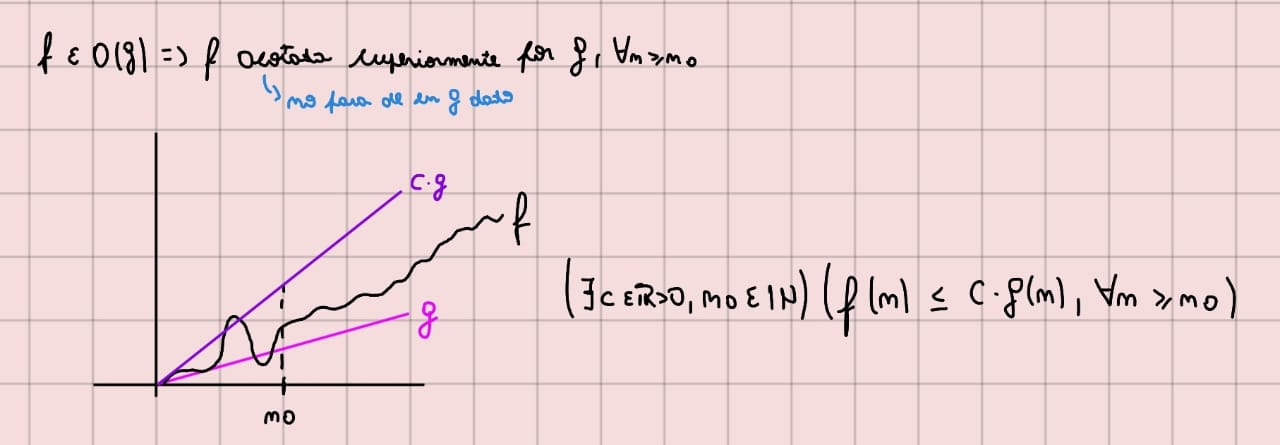
\includegraphics[width=\linewidth]{assets/notacion_o.png}
\end{minipage}\]
\subsection*{\(\Omega\) (cota inferior)}
Sirve para representar el límite o cota inferior del tiempo de ejecución de un algoritmo.
La notación f \(\in \Omega(g)\) expresa que la función f está acotada inferiormente por alguna función proporcional a g (g es cota inferior de f). \\
Ej: 100\(n^{2} + 300n + 1000 \in Omega(n^{2})\) \(\land\) 100\(n^{2} + 300n + 1000 \in Omega(n)\)
\begin{itemize}
    \item \(n/2 \in \Omega(n)\)
    \item \(n-1 \in \Omega(n)\)
    \item \(n^{2} \in \Omega(n)\)
    \item \(n^{k} \in \Omega(n)\) 
    \item \(log(n) \notin \Omega(n)\) 
\end{itemize}
\[\begin{minipage}[b]{0.5\textwidth}
    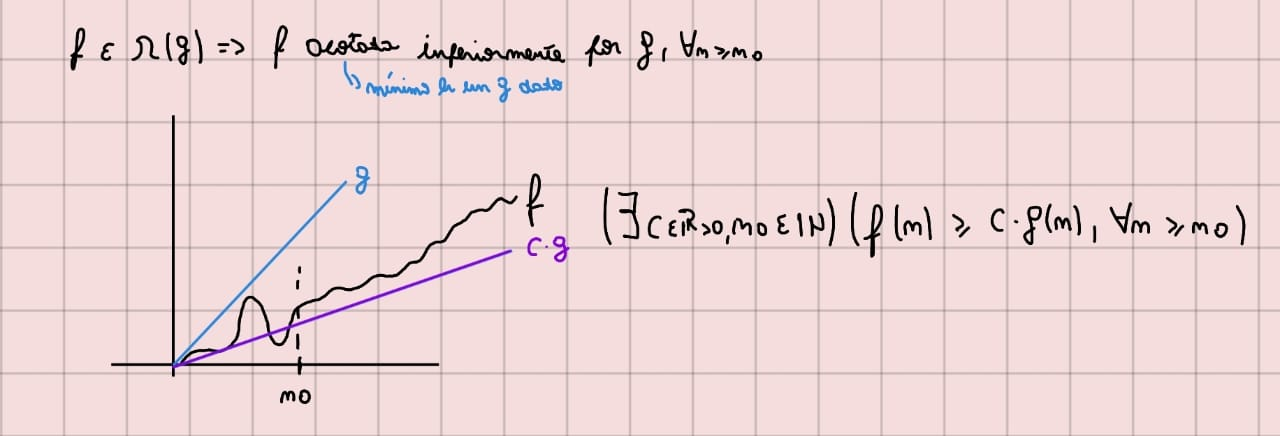
\includegraphics[width=\linewidth]{assets/notacion_omega.png}
\end{minipage}\]
\subsection*{\(\theta\) (orden exacto)}
\[f (n) \in \theta(g(n)) \iff f (n) \in O(g(n)) \ y \ f (n) \in \Omega(g(n)).\ Es \ decir, \ \theta(g(n)) = O(g(n)) \cap \Omega(g(n))\]
Básicamente: Tiene que valer en O y en \(\Omega\), no debe pasarse de \(\Omega\) pero tampoco estar por debajo de O.
\[\begin{minipage}[b]{0.5\textwidth}
    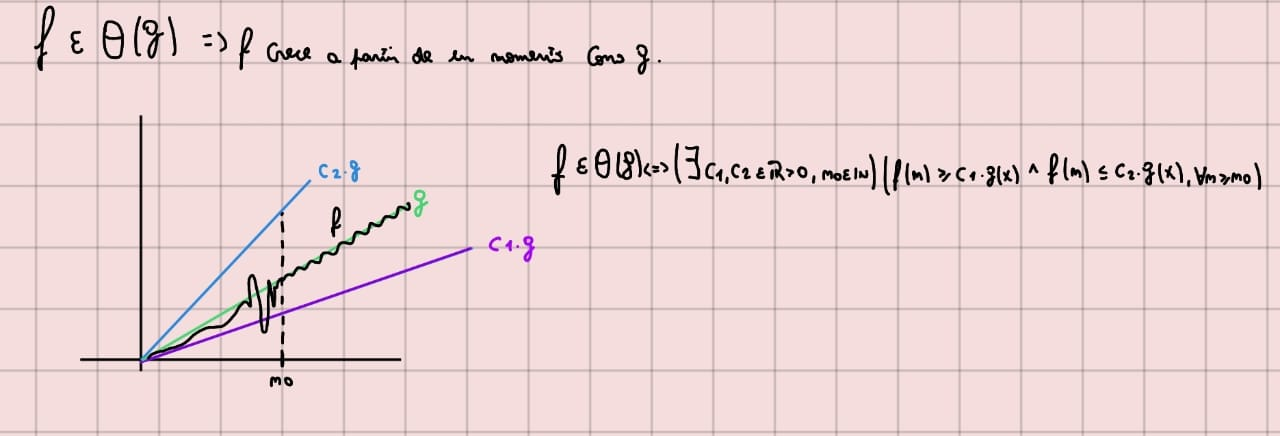
\includegraphics[width=\linewidth]{assets/notacion_theta.png}
\end{minipage}\]
\subsection*{Definición parecida a inducción corrida en Complejidad}
Tanto en la definición de \(O, \ \Omega \ y \ \theta\) se nombra para un \(n > n_{0}\). Esto es porque no todas las funciones cumplirán la definición, sino aquellas que son mayores a \(n_{0}\). Es por eso que en las imágenes se ven como inicialmente no cumple, pero a partir de un \(x_{0} \ (n_{0})\) vale para todo n.
\subsection*{Propiedades}
\begin{itemize}
    \item Suma: O(f) + O(g) = O(f+g) = O(max{f,g})
    \item Producto: O(f) \(\ast\) O(g) = O(f*g)
    \item Reflexividad: f \(\in O(f)\)
    \item Simetría: Solo vale en \(\theta\) = \(f \in \theta(g) \implies g \in \theta(f)\)
    \item Transitividad: \(f \in O(g) \land g \in O(h) \implies f \in O(h)\)
\end{itemize}
\subsection*{Intuición de Análisis de Complejidad posibles}
\begin{itemize}
    \item Mejor caso != Peor caso (cuando el ciclo corta antes)
    \item Mejor caso = Peor caso (cuando el ciclo no tiene condición de corte)
    \item Cuando tengo ramas if else, la complejidad mayor se dará por la rama que tenga mayor cantidad de operaciones en cuanto a ciclos.
    \item Cuando tenga guardas como por ejemplo, while $b>0$ y la variable se va dividiendo entre dos, la complejidad será algo parecida a log n.
    \item Cuando una función recibe dos parámetros, pero uno de ellos no tiene un rol fundamental en algún ciclo o guarda, entonces raramente esté en el cálculo final de la complejidad.
    \item Recordar que es normal ver casos donde se aplique la sumatoria de gauss o tengamos que masajear la expresión para que aparezca.
    \item Si la guarda del ciclo se incrementa de manera: $i*2$ o $i/2$ entonces la complejidad del ciclo será logarítmica.
    \item Para poder calcular la complejidad, si tenemos una suma basta con quedarnos con el término más grande. (ej: n + m tiene 2 casos)
\end{itemize}

\subsection*{Cota Ajustada}
Usamos \(\theta\) para indicar cotas ajustadas al momento de tener que calcular el peor y el mejor caso.
\subsection*{Complejidad Algorítmica en Polinomios}
Usamos límites para estos casos \\

Sean f, g: \(\mathds{N} \implies \float_{>0}\). Si existe:
\[ \lim_{n\to\infty} f(x)/g(n) = l \in \float_{\ge 0} \cup \{ +\infty \} \]
\begin{itemize}
    \item \(f \in \theta(g) \iff 0<l<+\infty\)
    \item \(f \in O(g) \ y \ f \notin \Omega(g) \iff l = 0\)
    \item \(f \in \Omega(g) \ y \ f \notin O(g) \iff l = +\infty\)
\end{itemize}
\section*{Complejidad en procedimientos de módulo}
Se calculan igual que observando una función dada que hace algo. Lo único que quería aclarar acá, es que siempre para las eliminaciones o búsquedas nunca se usen (en caso de haber) punteros que tengan referencia al último valor. El caso excepcional es el primero, pero el último hay que buscarlo con la forma de recorrer la estructura tradicional que haya. \\
Véase \hyperref[subsec:complejidad_modulo_sll]{anexo} para ver un ejemplo al respecto.
\section*{Árboles / Árboles binarios}
Se definen recursivamente y sus operaciones necesitan de ella. Utilizamos nodos. \\
Terminología que vamos a usar: Raíz \& Hoja \\ 
Para poder obtener un elemento de un árbol se debe empezar por la raíz y recorrer cada una de las hojas recursivamente. \\ \\
OBS: Las hojas pueden tener o no nodos hijos; si tienen hijos entonces también son árboles.  \\ 
\textbf{Árboles binarios}
Son aquellos en los cuales cada nodo tiene máximo 2 elementos.
\subsection*{Árboles binarios de búsqueda (ABB)}
Para todo nodo, los valores del subárbol izquierdo son menores que el valor del nodo y los valores del subárbol derecho son mayores. \\ 
\begin{minipage}[b]{0.8\textwidth}
    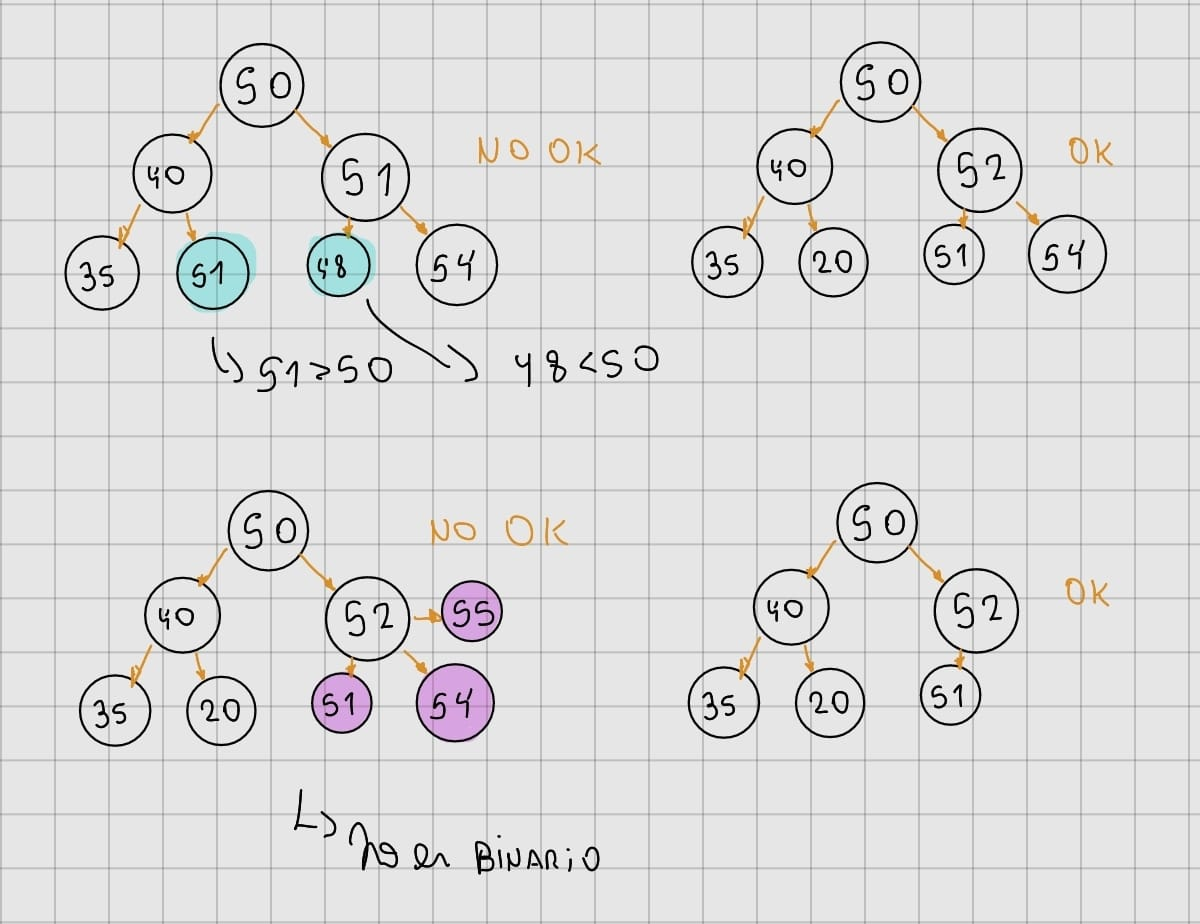
\includegraphics[width=\linewidth]{assets/abb-1.jpg}
    \centering
    \label{fig:abb-1}
\end{minipage} \\ 
Nótese que de ninguna rama derecha puede haber un número mayor a la raíz; de ninguna rama izquierda puede haber un número menor a la raíz. \\ 
La complejidad de búsqueda en el peor caso es de $O(log n)$
Algoritmos comúnes en árboles binarios de búsqueda:
\begin{itemize}
    \item Arbol vacío: Aquel que tiene la raíz en null
    \item Búsqueda de elemento: Si el nodo es null o el elem es igual al valor del nodo devuelvo n. Caso contrario, si el valor a buscar es menor al dato del nodo entonces busco más a la izquierda, caso contrario busco a la derecha. Cuando busca, habla de llamar a la misma función recursivamente. Complejidad O(n) con n la altura del árbol porque pasa solo una vez por cada nodo.
    \item Insertar elemento: Primero agarro la raiz del árbol, si la raiz es null entonces no hago nada. Si el árbol no tiene una raíz, entonces mi elem es la raíz; Si ya tiene una raíz me fijo si el elem a insertar es menor o mayor a la raíz, si es mayor entonces voy al primer hijo derecho de la raíz (no entiendo la parte final) dice algo como si el elem<prev.dato then padre.izq = newnodo osea tiene sentido pero en el pseudocodigo prev no existe enn ningun lado definido. Complejidad O(n) para agregar, aunque si hay distribución uniforme de las claves O(log n)
    \item Eliminar elemento: hay 3 casos. Sea u una variable cualquiera
    \begin{itemize}
        \item u es una hoja: Si u es una hoja significa que no tiene hijos, por lo tanto lo puedo eliminar sin necesidad de reordenar nada.
        \item u tiene un solo hijo: Si u es una hoja con un solo hijo (a la izq o a la derecha) basta con mover el hijo a la posición del nodo a eliminar.
        \item u tiene dos hijos: Si u es un nodo con dos hijos hay que encontrar al predecesor inmediato (v) de u. \textbf{v no puede tener dos hijos, en caso contrario no es predecesor inmediato}, una vez encontrado copiar la clave de v en lugar de la de u, borrar el nodo v (acá hay que revisar qué sucede si tiene un hijo, iría al caso 2, caso contrario caso 1). Lo mismo se puede hacer con el sucesor inmediato (mismas reglas que predecesor inmediato). 
        \item Complejidad O(n) para cualquier tipo de borrado.
    \end{itemize}
\end{itemize}
\textbf{Aclaración}: Predecesor inmediato (el más grande de los chiquitos), osea rama izquierda busco el último de la der a partir del nodo que estoy. \\ 
\textbf{Aclaración}: Sucesor inmediato (el más chiquito de los grandes), osea rama derecha busco el último a la izquierda a partir del nodo que estoy. \\
\subsection*{ABB con complejidad O(n) en ciertas operaciones}
Árbol binario con n nodos anidados todos mayores o todos menores.
\begin{center}
    \begin{minipage}[b]{0.7\textwidth}
        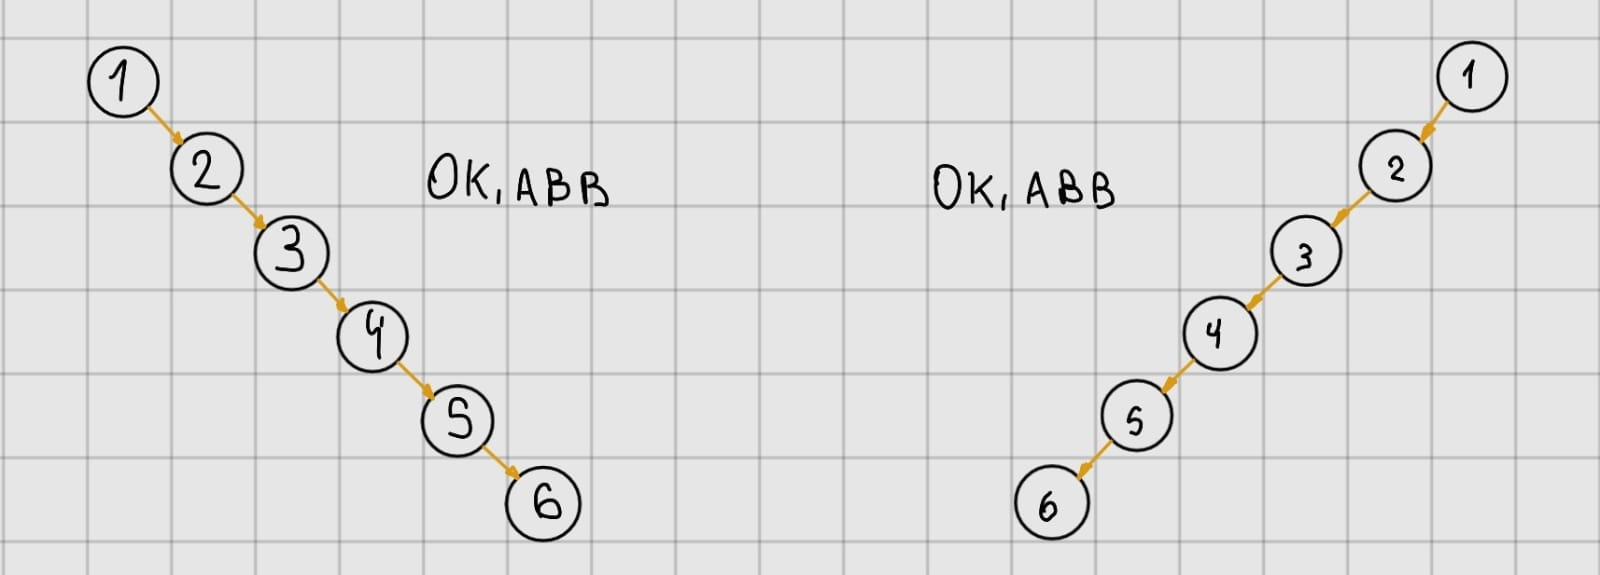
\includegraphics[width=\linewidth]{assets/peor_caso_abb.jpg}
        \centering
        \label{fig:peor_caso_abb}
    \end{minipage}
\end{center}
¿Cuál es el problema de los ABB? que al hacer inserciones, eliminaciones o ver si un elemento dado pertenece al árbol, el costo en el peor caso es O(n). \\ 
Para optimizar esto, existen los AVL que nos ponen restricciones en base a la cantidad de nodos que puede haber anidados en base ciertas reglas de balanceo.
\subsection*{ABB balanceados (AVL)}
Un árbol AVL es un ABB balanceado en altura. Un árbol binario perfectamente balanceado de n nodos tiene una altura de: $ log_{2}(n) + 1 $ donde las hojas son más del 50\% de los nodos  \\
La inserción y el borrado se hace exactamente igual que en un ABB pero acá, como extra se hace el rebalanceo. \\ 
Se define el factor de balanceo de un nodo v de un árbol binario como: \\
\[fb(v) = A_{D} - A_{I}\] donde $ A_{x}$ es la altura del subárbol x \\
Existen 3 posibles factores de balanceo para cada nodo: 
\begin{itemize}
    \item -1: La cantidad de ramas de la izquierda del nodo son más que la rama derecha.
    \item 0: La cantidad de ramas a la izquierda o derecha del nodo son la misma cantidad.
    \item 1: La cantidad de ramas de la derecha del nodo son más que la rama izquierda.
\end{itemize}
Llamamos entonces, árbol balanceado para cuando para cualquier nodo en él, la diferencia de longitud entre sus ramas izquierda y derecha difiere, a lo sumo, en una unidad. \\ 
\textbf{Nota: los caminos no nos importan mucho, considerar cada nodo como un árbol distinto. Si los tengo en misma altura pero uno está más abajo que otro, está desbalanceado. }
\begin{center}
    \begin{minipage}[b]{0.5\textwidth}
        \includegraphics[width=\linewidth]{assets/avl.png}
        \centering
        \label{fig:avl}
    \end{minipage}
\end{center}
\begin{itemize}
    \item Negro: Factor de balanceo 0.
    \item Rojo: Factor de balanceo -1.
    \item Azul: Factor de balanceo 1.
\end{itemize}
\subsection*{Mantener balanceo de AVL al insertar o eliminar}
Una de las dificultades más grandes de mantener el AVL invariante luego de cada operación es mantenerlo balanceado. \\
Viendo la figura de la izquierda: es un AVL porque si vemos, la rama de la izquierda del 10 son 2 nodos y la derecha 1 y difieren en un solo nodo, por lo tanto está balanceado. 
\begin{center}
    \begin{minipage}[b]{0.7\textwidth}
        \includegraphics[width=\linewidth]{assets/avl_problematica.png}
        \centering
        \label{fig:avl_problematica}
    \end{minipage}
\end{center}
Viendo la figura de la derecha, no está balanceado: porque la rama de la izquierda del 10 son 3 nodos (altura 3) y la derecha 1 (altura 1), y difieren en 2 nodos, por lo tanto no está balanceado. \\
¿Cómo solucionamos esto para mantener el invariante? Rotaciones
\newpage
\subsection*{Rotaciones}
Existen muchas rotaciones posibles para un árbol, pero las elegimos dependiendo de la estructura del árbol que tengamos que rebalancear. \\
Es importante que cada vez que hacemos una rotación, el invariante debe seguir valiendo. \\
\begin{center}
    \begin{minipage}[b]{0.7\textwidth}
        \includegraphics[width=\linewidth]{assets/avl_rotaciones.png}
        \centering
        \label{fig:avl_rotaciones}
    \end{minipage}
\end{center}
Nótese que al rotar el árbol, sigue valiendo el invariante que $ A < x < B < y < C $, esto nos indica que al rotar conseguimos el mismo árbol. \\ \\ 
\textbf{¿Qué rotación tengo que usar?}
\begin{itemize}
    \item Left-Left(LL o II): Ocurre cuando un nodo tiene un subárbol izquierdo que está desbalanceado a la izquierda. La solución es una rotación simple a la derecha. Véase \hyperref[subsec:rotaciones_avl]{anexo}
    \item Right-Right(RR o DD): Ocurre cuando un nodo tiene un subárbol derecho que está desbalanceado a la derecha. La solución es una rotación simple a la izquierda. Véase \hyperref[subsec:rotaciones_avl]{anexo}
    \item Left-Right(LR o ID): Ocurre cuando un nodo tiene un subárbol izquierdo que está desbalanceado a la derecha. La solución son dos rotaciones: primero una rotación a la izquierda en el subárbol izquierdo y luego una rotación a la derecha en el nodo. Véase \hyperref[subsec:rotaciones_avl]{anexo} 
    \item Right-Left(RL o DL): Ocurre cuando un nodo tiene un subárbol derecho que está desbalanceado a la izquierda. La solución son dos rotaciones: primero una rotación a la derecha del subárbol derecho y luego una rotación a la izquierda en el nodo. Véase \hyperref[subsec:rotaciones_avl]{anexo}
\end{itemize}
Consejos útiles:
\begin{itemize}
    \item Muchas veces, una rotación no siempre es suficiente para rectificar un nodo que está desequilibrado. 
    \item El rebalanceo (realiza las rotaciones) se invoca para todos los nodos de la rama hasta la raíz (hay que mandar el árbol entero).
    \item El máximo de rotaciones consecutivas para balancear un árbol es de 2.
    \item Al insertar un nodo en un AVL, el costo es O(log n). El costo de inserción es O(log n) y luego para rebalancear tambien, O(log n).
\end{itemize}
\begin{center}
    \begin{minipage}[b]{0.7\textwidth}
        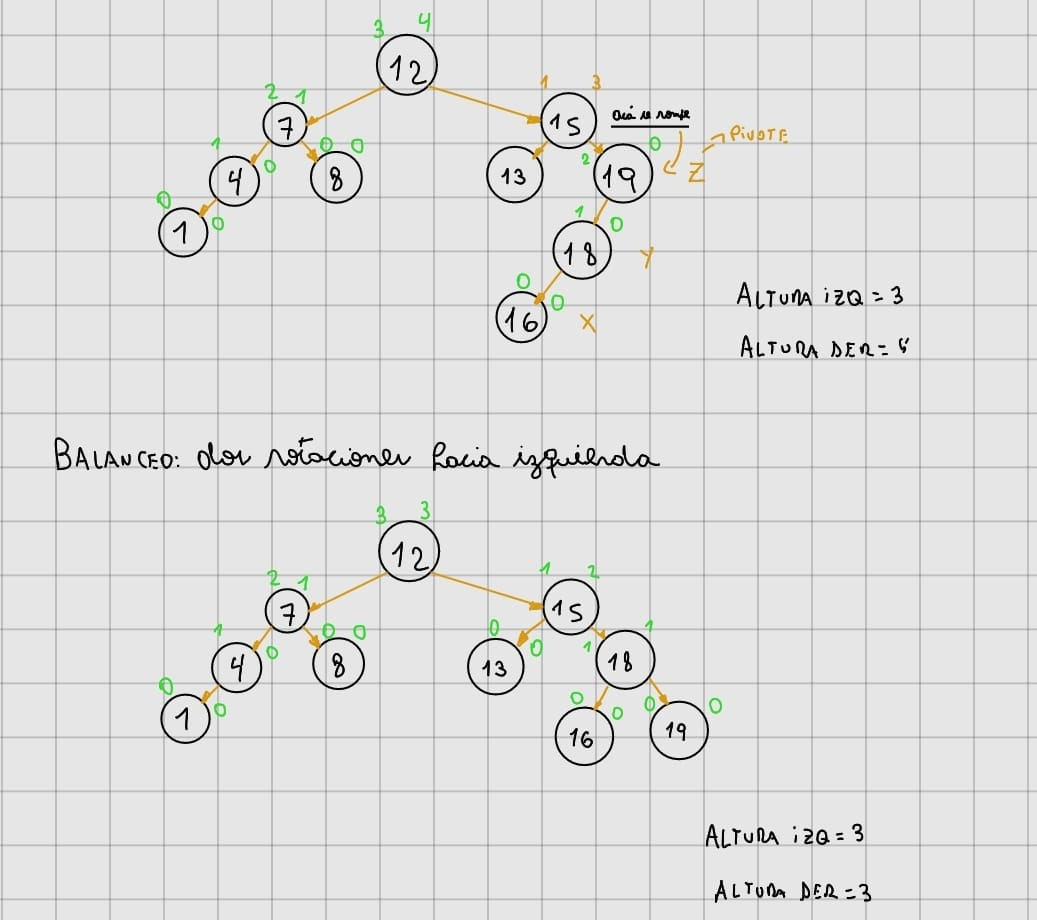
\includegraphics[width=\linewidth]{assets/balanceo_avl.jpg}
        \centering
        \label{fig:balanceo_avl}
    \end{minipage}
\end{center}
\section*{Cola de Prioridad}
Es exactamente igual que el TAD Cola, pero difiere en la forma en que removemos elementos. No quitamos el primero que ingresó, sino que lo sacamos en base a un factor de prioridad que definimos a la hora de armar el TAD. \\ 
Si llegase a suceder que un mismo elemento tiene la misma prioridad, debería especificarse cual se quitaría. \\ 
La prioridad la expresamos con un entero, pero puede ser cualquier tipo $ \alpha$ que pueda ser comparado con un orden $<_{\alpha}$. \\

\textbf{Ej.}: Imaginemos que vamos a una guardia, y estamos primeros a punto de ser atendidos pero llega alguien que está en estado grave. Esta persona va a ser atendida antes que nosotros aunque hayamos llegado antes. En ese caso, es una cola de prioridad pues la prioridad está dada por la gravedad del paciente. \\ \\ 
Casos de uso: 
\begin{itemize}
    \item Sistemas operativos
    \item Algoritmos de Scheduling
    \item Gestión de colas
\end{itemize}
Véase \hyperref[subsec:cola_de_prioridad_avl]{\underline{anexo}} para un ejercicio de elección de estructuras para armar una cola de prioridad.
\section*{Heaps}
Es la implementación del TAD ColaPrioridad. Tiene la misma complejidad algorítmica que un árbol AVL pero es más fácil y elegante de implementar. \\
Invariante de representación:
\begin{itemize}
    \item Árbol binario perfectamente balanceado (difiere a lo mucho en un único nodo)
    \item El último nivel está lleno de nodos desde la izquierda (es izquierdista). Cuando el nivel del la rama izquierda ya difiere en uno con la derecha, agrego en las hojas de la rama derecha para dejar el árbol con misma altura, pero la idea es agregar de izquierda a derecha siempre. 
    \item La clave (prioridad) de cada nodo es \textbf{mayor o igual} que la de sus hijos (si es que tiene)
    \item Todo súbarbol es otro heap. 
    \item NO es un ABB. En un ABB el hijo derecho es más grande que el padre. En un Heap ambos hijos de un Nodo son menores.
\end{itemize}
Min-Heap: Min hace referencia a que el proceso de extraer, se hace sacando el mínimo en O(1). Si sacamos el mínimo en O(1) significa que todos los nodos debajo de la raíz son menores estrictos a él. \\
Max-Heap: Max hace referencia a que el proceso de extraer, se hace sacando el máximo en O(1). Si sacamos el máximo en O(1) significa que todos los nodos debajo de la raíz son mayores estrictos a él. \\

Véase \hyperref[subsec:operaciones_heaps]{\underline{operaciones heaps}} para un ejemplo más visual de las operaciones \\
Véase \hyperref[subsec:implementaciones_heap]{\underline{implementaciones heaps}} de maneras diversas.
\subsection*{Complejidad en operaciones con Heaps}
Nota: acá hablamos de un max-heap. recordemos que los que están arriba son mayores estrictos que los hijos.
\begin{itemize}
    \item Próximo: O(1) $\rightarrow$ raíz del árbol o primer elemento del array.
    \item Encolar(elemento): O(log n) $\rightarrow$ Sin necesidad de conocer el elemento, lo que tenemos que tratar es llenar el árbol de manera izquierdista. Hay dos casos
    \begin{itemize}
        \item Si el elemento que ingresé en el lugar libre es \textbf{menor a su padre, dejo todo como está.}
        \item Si el elemento que ingresé en el lugar libre es mayor a su padre, \textbf{hago el swap con el padre}. Por lo tanto ahora tengo garantizado que el elemento nuevo es el padre y los hijos son menores a este (vuelve a valer el invariante).
        \item \textbf{Algoritmo}: Insertar elemento al final del heap, y luego subir(elemento)
    \end{itemize}
    \item Subir(elemento) o Sift-Up: Mientras que el elemento no sea la raíz, y la prioridad del elemento sea mayor al padre, entonces intercambio \textbf{el elemento con el padre}.
    \item Desencolar(elemento): O(log n) $\rightarrow$ Son varios pasos 
    \begin{itemize}
        \item Intercambio la raíz con el último elemento ingresado. 
        \item Borro mi anterior raíz.
        \item Mi nueva raíz (el último ingresado), lo comparo con sus dos hijos verificando que 
        \begin{itemize}
            \item si estamos en un max-heap, sea el mayor de los dos hijos, si no lo es, entonces intercambio con el MAYOR/IGUAL HIJO. Hago esto recursivamente. 
            \item si estamos en un min-heap, sea el menor de los dos hijos, si no lo es, entonces intercambio con el MENOR/IGUAL HIJO. Hago esto recursivamente. 
        \end{itemize} 
    \end{itemize} 
    \item Bajar(p): Mientras que p no sea hoja y la prioridad de p sea menor al mayor de sus hijos, intercambio el hijo con p.

\end{itemize}
\subsection*{Transformaciones Array a Heap}
Véase \hyperref[subsec:array_2_heap]{\underline{array $\rightarrow$ heap}}
\section*{Tries}
El Trie es una estructura de datos que se suele utilizar en autocompletado de texto, pattern matching, etc.  \\
La principal característica es que la complejidad depende del tamaño de los elementos (en general, palabras) y no de la cantidad de elementos.
\begin{itemize}
    \item Se implementa sobre árboles n-arios: Donde n sería el tamaño del alfabeto más uno (por el símbolo reservado \$)
    \item Se usan para guardar grandes conjuntos de palabras o secuencias de elementos con un alfabeto reducido
    \item Cada nodo representa un caracter o componente de los elementos guardados.
    \item Se marca con \$ la finalización de la palabra o elemento. Donde el significado \$ es el valor de la palabra entera.
    \begin{itemize}
        \item El camino de la carrera Análisis I, en el valor de I el significado podría ser un objeto de esa materia.
    \end{itemize}
    \item Los caracteres, se van colocando donde se desea completar la palabra, pero no puede tener un hijo derecho y sí un hijo izquierdo.
\end{itemize}
\begin{center}
    \begin{minipage}[b]{0.6\textwidth}
        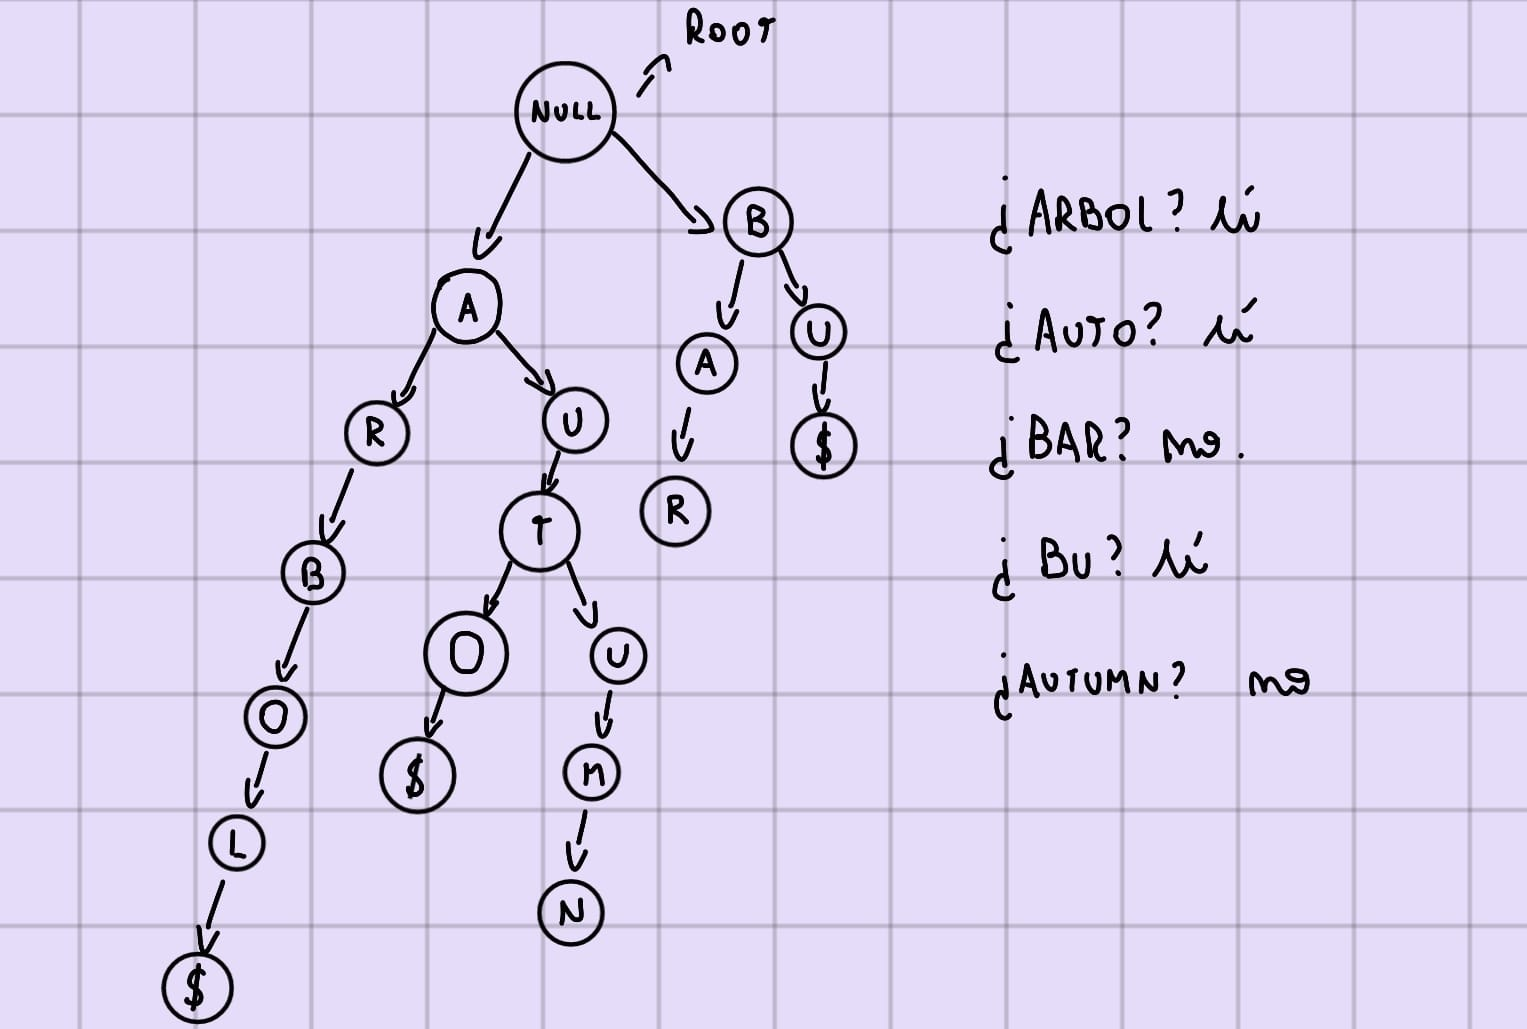
\includegraphics[width=\linewidth]{assets/trie.jpg}
        \centering
        \label{fig:trie}
    \end{minipage}
\end{center}
Propiedades:
\begin{itemize}
    \item En el nivel i-ésimo del árbol se guarda en el i-ésimo componente de la palabra/secuencia.
    \item La estructura del trie es única, no importa el orden en que se ingresen los valores de los nodos.
    \item Complejidad o(m) donde m es la longitud de la cadena involucrada en el procedimiento.
    \item La raíz de todo Trie es nulo, porque es la palabra vacía.
    \item Las palabras, terminan con \$. Si no hay un camino que termine con \$ entonces no es una palabra válida. 
\end{itemize}
Nota: Hay muchos algoritmos de Trie que tienen buena complejidad temporal pero son muy malos en complejidad espacial.
\section*{Hashing}
Refiere al proceso de tomar una entrada, de cualquier tipo y generar una cadena de caracteres de longitud fija que representa de manera única esta entrada. \\
Son adecuados para representar diccionarios y/o conjuntos. \\
\subsection*{Representación}
Representemos un diccionario con
\begin{itemize}
    \item Tupla $<T, h>$ donde T es un arreglo con N = tamaño(T) celdas
    \item $h \ es \ una \ funcion \ hash:h(k) \rightarrow {0,..., n-1}$
    \begin{itemize}
        \item k: Conjunto de claves posibles 
        \item {0, ..., n-1}: Conjunto de las posiciones de la tabla (pseudoclaves)
        \item Para poder conseguir la posición de un elemento en el arreglo usamos la función h.
    \end{itemize}
\end{itemize}
\subsection*{Colisiones}
Las colisiones en un hash ocurre cuando dos entradas (keys) distintas producen el mismo valor de hash. \\
Un algoritmo de hash debería producir hashes únicos para cada entrada, sin embargo, debido a las limitaciones en la longitud finita de los hashes y a la naturaleza de la función hash es matemáticamente inevitable que ocurran colisiones en algún momento. \\
\textbf{Un buen algoritmo de hash minimiza la probabilidad de colisiones} \\
Maneras de resolver colisiones:
\begin{itemize}
    \item Direccionamiento Cerrado / Encadenamiento: Cada celda de la tabla hash mantiene una lista enlazada de todos los elementos que han colisionado en esa celda. En el mejor caso, el facotr de carga $\alpha =$ cantidad de elementos/cantidad de posiciones. Las operaciones sobre la listas enlazadas tendrán $\Omega(N/\longitud{T})$ y $O(N)$ 
    \begin{center}
        \begin{minipage}[b]{0.5\textwidth}
            \includegraphics[width=\linewidth]{assets/hashing_le.png}
            \centering
            \label{fig:hashing_le}
        \end{minipage}
    \end{center}
    \item Direccionamiento abierto: Cuando ocurre una colisión, se busca otra ubicación vacía dentro de la tabla hash para almacenar el elemento adicional. Este método puede producir deslocalización del elemento ya que cuando vuelva a llamar a la clave, el valor de hash para esa clave no va a coincidir con la posición del elemento, sino que habrá que hacer el mismo recorrido a la hora de setearlo. 
    \begin{center}
        \begin{minipage}[b]{0.5\textwidth}
            \includegraphics[width=\linewidth]{assets/hashing_posicion_vacia.png}
            \centering
            \label{fig:hashing_posicion_vacia}
        \end{minipage}
    \end{center}
\end{itemize}
\subsection*{Barridos}
También conocido como "scanning in hashing", se refiere a la acción de recorrer toda la tabla hash en búsqueda de un elemento específico o en caso de una colisión. Los barridos se diferencian por su complejidad algorítmica.
\begin{itemize}
    \item Barrido lineal: Cuando ocurre una colisión el algoritmo busca secuencialmente la siguiente ubicación disponible en la tabla hash hasta encontrar una celda vacía.
    \begin{itemize}
        \item Fórmula para encontrar la siguiente ubicación: $h(k, i) = (h'(k)+i) \ mod \ m$
        \item h(k, i) = nueva función hash 
        \item h'(k) = función hash original
        \item i = número de intentos de búsqueda 
        \item m = tamaño de la tabla hash
        \item Los elementos se aglomeran por largos tramos y puede surgir \textbf{aglomeración primaria}.
    \end{itemize}
    \item Barrido cuadrático: El incremento de las iteraciones es cuadrático.
    \begin{itemize}
        \item Fórmula para encontrar la siguiente ubicación: $h(k,i) = (h'(k) + c_{1} \ast i + c_{2} \ast i^{2}) \ mod \ m$
        \item El barrido cuadrático reduce el agrupamiento que a veces ocurre con el barrido lineal, sin embargo, puede sufrir de agrupamientos cuadráticos si no se eligen adecuadamente las constantes de incremento.
        \item El agloramiento para este barrido se llama \textbf{aglomeración secundaria}
    \end{itemize}
    \item Hashing doble: Se utiliza una segunda función de hash para calcular una ubicación alternativa cuando ocurre una colisión 
    \begin{itemize}
        \item Fórmula para encontrar la siguiente ubicación: $h(k, i) = (h_{1}(k) + i \ast h_{2}(k)) \ mod \ m$
        \item Donde $h_{1}(k) \ y \ h_{2}(k)$ son dos funciones de hash diferentes
        \item i = número de intentos de búsqueda 
        \item m = tamaño de la tabla hash
        \item El uso de una segunda función de hash reduce las posibilidades de agrupamiento y mejora la distribución de las claves en la tabla hash. 
        \item No se generan esas aglomeraciones o clusters tan frecuentes.
    \end{itemize}
\end{itemize}
\subsection*{Requisitos para una función hash}
\begin{itemize}
    \item Determinismo: Dada una misma entrada, la salida debe ser siempre el mismo hash.
    \item Eficiencia: Debe ser rápido de calcular.
    \item Difusión: Pequeños cambios en la entrada deberían producir cambios significativos y difíciles de predecir en el valor hash. 
    \item No reversibilidad: No se debe ser posible obtener el valor orignal a partir del hash. 
    \item Unicidad: Cada entrada debería producir un hash único. Es decir, no debería haber dos entradas diferentes con el mismo hash (ej: uuid)
    \item Uniformidad de distribución: Los valores hash deberían estar distribuidos uniformemente a lo largo del espacio de salida posible. Esto mejora la eficiencia del hashing y reduce la probabilidad de colisiones
\end{itemize}
\section*{Anexo}
\subsection*{Ejemplo 1 en cálculo de complejidad}
\begin{lstlisting}
    void add(int mat1[n][n], mat2[n][n]){
        int ans[n][n];
            for(int i = 0; i < n; i++){
                for(int j = 0; j < n; j = j+1){
                    ans[i][j] = mat1[i][j] + mat2[i][j];
                }
            }
        return ans[0][0];
    }
\end{lstlisting}
$\textbf{Parte 1}$: Comenzamos colocando la cantidad de operaciones que se realizan, línea a línea. Los ciclos, en el caso del for, posee 3 casos: el caso inicial, caso intermedio, caso fin.
\begin{lstlisting}
    void add(int mat1[n][n], mat2[n][n]){
    0    int ans[n][n];
    2 2 2   for(int i = 0; i < n; i++){
    2 3 3       for(int j = 0; j < n; j = j+1){
    8               ans[i][j] = mat1[i][j] + mat2[i][j];
                }
            }
    3    return ans[0][0];
    }
\end{lstlisting}
Obs: j = j+1 $\neq$ j++ en temas de cantidad de operaciones. El j++ es una operación menos aunque hagan lo mismo.
Obs: El return funciona como una asignación, por lo tanto también cuenta en operaciones. \\
$\textbf{Parte 2}$: Elegimos si empezamos por el mejor, o el peor caso. El peor caso suele ser el más tedioso así que empecemos por ese. \\
$\textbf{Parte 2.1: Peor caso}$ \\
$\textbf{Parte 2.1.1 }$: Empezamos considerando el caso intermedio del ciclo.
\begin{lstlisting}
    2 3 3   for(int j = 0; j < n; j = j+1){
    8           ans[i][j] = mat1[i][j] + mat2[i][j];
            }
\end{lstlisting}
$ \sum_{j=0}^{n-1}{(8+3)} $ \\
Ahora consideramos el caso inicial del ciclo, y el final: $ 2 + \sum_{j=0}^{n}{(8+3)} + 3$ \\
Definimos:  $a \equiv 2 + \sum_{j=0}^{n-1}{(8+3)} + 3$ \\
$\textbf{Parte 2.1.2}$: 
\begin{lstlisting}
2 2 2   for(int i = 0; i < n; i++){
            a
        }
\end{lstlisting}
Comenzamos considerando el caso intermedio del ciclo.
$ \sum_{i=0}^{n}{(a+2)} $ \\
Ahora consideramos el caso inicial del ciclo, y el final:
$ 2 + \sum_{i=0}^{n}{(a+2)} + 2 $ \\ 
Definimos:  $b \equiv 2 + \sum_{i=0}^{n-1}{(a+2)} + 2 $ \\
$\textbf{Parte 2.1.3}$: Juntar ambos ciclos
$c \equiv 2 + \sum_{i=0}^{n-1}{((2 + \sum_{j=0}^{n-1}{(8+3)} + 3)+2)} + 2 $ \\ 
$\textbf{Parte 2.4}$: Resolver los ciclos, uniéndolos de alguna forma \\
$\equiv 2 + \sum_{i=0}^{n-1}{((2 + \sum_{j=0}^{n-1}{(\textbf{8+3})} + 3)+2)} + 2 $ \\ 
$\equiv 2 + \sum_{i=0}^{n-1}{((\textbf{2} + \sum_{j=0}^{n-1}{11} + \textbf{3})+2)} + 2 $ \\ 
$\equiv 2 + \sum_{i=0}^{n-1}{((\sum_{j=0}^{n-1}{\textbf{11}} + 5)+2)} + 2 $ \\ 
$\equiv 2 + \sum_{i=0}^{n-1}{((11 * \sum_{j=0}^{n-1}{1} + 5)+2)} + 2 $ \\
$\equiv \textbf{2} + \sum_{i=0}^{n-1}{((11 * n + 5)+2)} + \textbf{2} $ \\  
$\equiv 4 + \sum_{i=0}^{n-1}{(11 * n + 5+2)} $ \\  
$\equiv 4 + \sum_{i=0}^{n-1}{(11 * n + 7)} $ \\
$\equiv 4 + n * (11 * n + 7) $ \\    
$\equiv 4 + 11n^{2} + 7n $ \\   
$\textbf{Parte 2.1.5}$: Agregar el caso del return 
$\equiv 3 + 4 + 11n^{2} + 7n $ \\   
$\equiv 11n^{2} + 7n + 7 $ \\
$\textbf{Parte 2.1.6}$: Observar cual es la variable con mayor exponente.
En este caso, es $11n^{2}$ por lo tanto, $T{peor}(n) = \Theta(max\{11n^{2}, n, 7\})$. Luego,  
$T{peor}(n) = \Theta(n^{2})$ \\ 
Nota: En la materia no utilizan los números de operaciones, pero acá por ejemplo 2, 8, 3, 3, 2 (operaciones elementales) serían $\Theta(1)$, osea nuestro cálculo de la Parte 2.1.5 se vería así: $\Theta(n^{2}) + \Theta(n) + \Theta(1)$ \\ 
$\textbf{Parte 2.2: Mejor caso}$ \\ 
El mejor caso es igual al peor caso porque no tenemos restricciones del ciclo más que las matrices de entradas y tampoco tenemos ninguna condición de corte. Siempre se recorre la misma cantidad de veces.
\subsection*{Ejemplo 2 en cálculo de complejidad}
\begin{lstlisting}
   int russian(int a, int b){
        int res = 0;
        while(b > 0){
            if(b % 2 == 1){
                res = res + a;
            }
            a = a * 2;
            b = b/2;
        }
        return res;
   }
\end{lstlisting}
A simple vista podemos notar algo, estamos usando un while y la guarda depende de un b que desconocemos. Veamos como va variando la variable b; Se observa que se va dividiendo por dos, entonces es algo más rápido que hacer b-1. Seguramente, el peor caso sea logarítmico (como en búsqueda binaria que se va partiendo la lista en dos)
\newpage
\textbf{Parte 1}: Comenzamos colocando la cantidad de operaciones que se realizan, línea a línea. 
\begin{lstlisting}
    int russian(int a, int b){
        1    int res = 0;
        1    while(b > 0){
        2        if(b % 2 == 1){
        2           res = res + a;
                 }
        2        a = a * 2;
        2        b = b/2;
            }
        1   return res;
    }
 \end{lstlisting}
$\textbf{Parte 2}$: Elegimos si empezamos por el mejor, o el peor caso. El peor caso suele ser el más tedioso así que empecemos por ese. \\
$\textbf{Parte 2.1: Peor caso}$ \\
$\textbf{Parte 2.1.1}$: Observamos que nuestro peor caso es que b $>$ 0 y al dividir b por 2 sea impar. \\ Dentro del ciclo tenemos: (1 + (2+2) + 2 + 2) operaciones elementales. \\
Nótese que el 1 es de la condición de la guarda. \\ 
El ciclo es algo inverso, se comienza siendo algo muy grande y se va achicando, y el ciclo termina cuando b = 0. ¿Cuantas veces tengo que dividir b entre 2 para que podamos llegar a 0? El logaritmo base 2 de b, pero acá b lo llamamos n. \\ 
$\textbf{Parte 2.1.2}$: Utilizar logaritmo para hablar del ciclo \\
$\log(n)(1+(2+2) + 2 + 2)$ \\
Nótese que eliminamos la base 2 porque en complejidad, la base del logaritmo da igual.  \\
$\textbf{Parte 2.1.3}$: Considerar la asignación inicial y el return junto al ciclo \\ 
$1 + \log(n)(1+(2+2) + 2 + 2) + 1 \equiv 1 + \log(n)(8) + 1$ \\ 
\textbf{Parte 2.1.4}: Calcular la complejidad
$T_{peor}(n) = \Theta(1) + \Theta(log(n)) + \Theta(1) \equiv \Theta(max\{1, log(n), 1\}) \equiv \Theta(log(n)) $ \\
\textbf{Parte 2.2: Mejor caso} \\
Si b = 0 inicialmente, no entra nunca al ciclo por lo tanto no hay complejidad alguna porque todas son operaciones elementales. \\
$T_{mejor}(n) = \Theta(1) + \Theta(1) + \Theta(1) \equiv \Theta(max\{1, 1, 1\}) \equiv \Theta(1)$ \\
\subsection*{Ejemplo 3 en cálculo de complejidad}
\begin{lstlisting}
    function AlgoritmoQueHaceAlgo(arreglo A)
    int i : = 1; int j := 1;
    int suma := 1; int count := 0;
    while i <= tam(A) do 
        if i != A[i] do 
            count : = count + 1;
        end if 
        j := 1;
        while j <= count do 
            int k := 1;
            while k <= tam(A) do 
                suma := suma + A[k];
                k := k * 2;
            end while 
            j := j+1;
        endwhile 
        i := i + 1;
    endwhile
    return suma
\end{lstlisting}
Lo primero que comenzamos viendo cual es el peor caso de las variables. \\
El ciclo más de adentro con guarda k depende del tamaño de A, por lo tanto el ciclo itera máximo $log(|A|)$ veces (xq k se va duplicando en cada caso). \\
El ciclo con guarda $j <= count$ depende de una variable count. En el peor caso ¿qué valor toma count? bueno, count se incrementa en el peor caso hasta ser $count = |A|$. Una observación importante es que count crece igual que |A| pero el proceso lo hace pasando por i = 0, i = 1 SIEMPRE. \\
El ciclo más de afuera con guarda i depende del tamaño de A, por lo tanto el ciclo itera máximo $|A|$ veces (xq empieza desde i = 1). \\
Luego, quedaría algo así: \\
$ \Theta(1) + \Theta(1) + (\sum_{i=0}^{|A|}{\Theta(1) + \Theta(1) + \Theta(1) + (\sum_{j=1}^{i}{\Theta(1) + (\sum_{k=0}^{log(|A|)}{\Theta(1) + \Theta(1)}) + \Theta(1)})} + \Theta(1)) + \Theta(1)  $ \\
$ \equiv \Theta(1) + \Theta(1) + (\sum_{i=0}^{|A|}{\Theta(1) + \Theta(1) + \Theta(1) + (\sum_{j=1}^{i}{log(|A|) \ast \Theta(1)})} + \Theta(1)) + \Theta(1) $ \\ 
$ \equiv \Theta(1) + \Theta(1) + (\sum_{i=0}^{|A|}{\Theta(1) + \Theta(1) + \Theta(1) + (\sum_{j=1}^{i}{log(|A|) \ast \Theta(1)})} + \Theta(1)) + \Theta(1) $ \\ 
$ \equiv \Theta(1) + \Theta(1) + (\sum_{i=0}^{|A|}{\Theta(1) + \Theta(1) + \Theta(1) + i * log(|A|)} + \Theta(1)) + \Theta(1) $ \\ 
$ \equiv \Theta(1) + (\sum_{i=0}^{|A|}{i * log(|A|)}) \leftarrow $ Como i depende del ciclo, lo dejo adentro pero saco lo demás hacia afuera.  \\ 
$ \equiv \Theta(1) + (log(|A|) * \sum_{i=0}^{|A|}{i}) $ \\ 
$ \equiv \Theta(1) + log(|A|) * |A|(|A|+1)/2  $ \\ 
$ \equiv log(|A|) * |A|^{2}/2 + |A|/2  $ \\ 
$ \equiv log(|A|) * |A|^{2}/2 + log(|A|) * |A|/2   $ \\ 
$ \equiv log(|A|) * |A|^{2} + log(|A|) * |A|  \leftarrow $ Saco denominadores, son constantes. \\ 
$ \equiv log(|A|) * |A|^{2} $ \\ 
$ \equiv \Theta(log(|A|) * |A|^{2}) $ \\
Conclusión: Es importante revisar que si el ciclo depende de una guarda como $ j \le count$ revisar como va creciendo count; como count depende del valor de i, i va siendo 1, 2, 3, 4, osea que no sucede una sola vez y no podemos generalizar. El peor caso sería que i pase por 1, 2, 3, 4, hasta tam(A), entonces el ciclo que depende de count se ejecuta 1 vez, despues 2 veces, después 3 y así.
\subsection*{Ejemplo 3 en cálculo de complejidad}
Recuerdo:
\begin{itemize}
    \item $\Theta(n)$: Cota ajustada, exactamente n. 
    \item $\Omega(n)$: Funciones mayores a n.
    \item $O(n)$: Funciones menores a n.
    \item c: Variable real mayor a 0. Nos basta con que exista una. 
    \item n: Mayor a n0 donde ambas son naturales, donde n es suficientemente grande.
\end{itemize}
Determine la verdad o falsedad de las siguientes afirmaciones: \\ \\ 
\textbf{1.} $ 2^{n} = O(1) $ \\
Para empezar, la igualdad de una función con un grupo de funciones significa lo siguiente $ 2^{n} \le c \ast 1 $ \\ 
Luego, $ 2^{n} = c $ es claramente es falso. \\ 
Contraejemplo: $ n = 4, 2^4 \neq O(1)$ \\ \\
\textbf{2.} $ n = O(n!) $ \\
Esperaría que sea verdadero porque es cierto que el conjunto de funciones menores a n! incluye a n.
$ n \le c * n!$ \\
$ n \le c * (n-1)! * n$ \\
$ 1 \le c * (n-1)! \leftarrow $ trivialmente verdadero para n suficientemente grande y c mayor que cero.\\ \\
\textbf{3.} $ n+m = O(nm) $ \\
Sabemos que n y m son dos valores de salida de una función. Parecería verdadero que una multiplicación de dos cosas incluya a la suma de ambas. \\
$ n+m \le c * nm $ \\
$ n/nm + m/nm \le c $ \\
$ 1/m + 1/n \le c \leftarrow $ trivialmente verdadero porque un $c>0$ siempre va a ser mayor a dos racionales que tienden a 0. \\ \\ 
\textbf{4.} $ f \in O(log \ n) \ entonces \ f \in O(n) $ \\
Esto es trivialmente verdadero a la vista porque sabemos que si f es una función que es menor a O(log n) entonces obligatoriamente f es menor a O(n) por transitividad $ \implies f \le O(log \ n) \le O(n) $ \\ \\  
$ f \in O(log \ n) \equiv f \le c * log(n), \ f \in O(n) \equiv f \le c * n $ \\
$ \implies f \le c * log(n) \implies f \le c * n $ \\
$ \implies c * log(n) \le c * n $ \\
$ \implies log(n) \le n \leftarrow $ trivialmente verdadero.
\newpage
\subsection*{Single Linked List - Complejidad - Implementación}
\label{subsec:complejidad_modulo_sll}
\begin{lstlisting}
    Struct NodoLista<T> {
        prev: NodoLista<T>
        sig: NodoLista<T>
        val: T
    }

    Módulo LinkedList<T> implementa Secuencia<T> {
        var primero: NodoLista<T>
        var ultimo: NodoLista<T>
        var longitud: int

        Costo peor caso / mejor caso = O(1) xq ya tengo primer puntero y lo peor que tengo que hacer es reordenar 1 solo. 
        proc agregarAdelante(inout l: LinkedList<T>, in e: T) {
            var nuevoNodo: NodoLista<T> = new NodoLista<T>(e);
            var primeroAnt: NodoLista<T> = l.primero;
            nuevoNodo.sig = primeroAnt;
            l.primero = nuevoNodo;
            if(l.longitud == 0){
                l.ultimo = nuevoNodo; 
            }
            l.longitud+=1;
        }

        Costo peor caso / mejor caso = O(1) xq ya tengo el último puntero y lo peor que tengo que hacer es reordenar 1 solo.
        proc agregarAtras(inout l: LinkedList<T>, in e: T){
            if(l.longitud == 0) then
                agregarAdelante(l, e);
            else
                var nuevoNodo: NodoLista<T> = new NodoLista<T>(e);
                var anteriorUlt: NodoLista<T> = l.ultimo; 
                anteriorUlt.sig = nuevoNodo; 
                l.ultimo = nuevoNodo; 
            endif
        }
        
        proc buscar(in l: LinkedList<T>, in e: T): T {
            // Si e == l.primero.val -> costo O(1)
            //Si e NO es el primero, entonces -> costo O(n)

            Aunque tenga el último guardado, no puedo sacarlo como caso aparte porque para calcular la complejidad tendría que aíslar los casos del primero y el último y es un quilombo.
        }
    }
\end{lstlisting}
\subsection*{Rotaciones según desbalance de AVL}
\label{subsec:rotaciones_avl}
\begin{center}
    \begin{minipage}[b]{0.9\textwidth}
        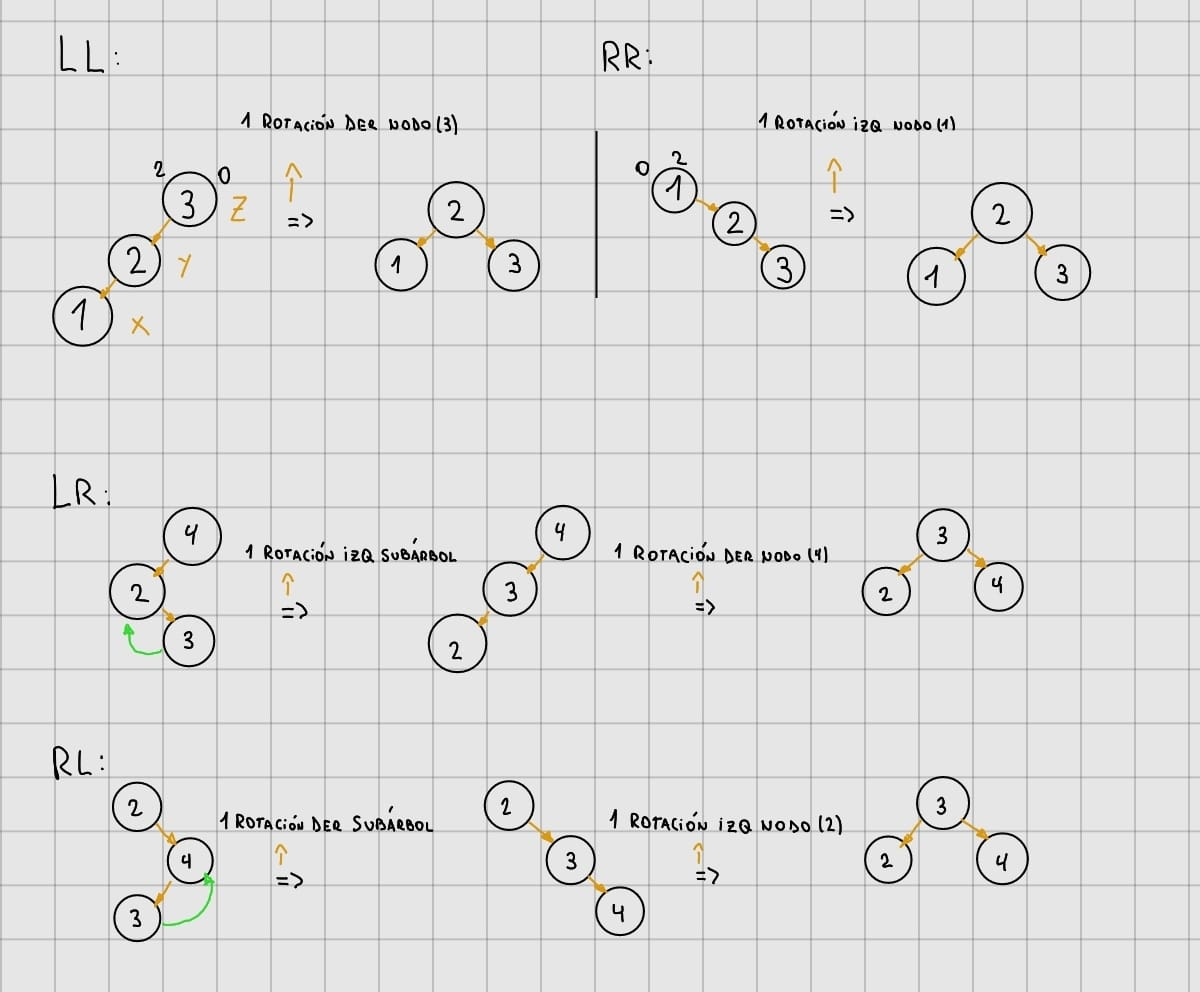
\includegraphics[width=\linewidth]{assets/rotaciones_avl_casos.jpg}
        \centering
        \label{fig:rotaciones_avl_casos}
    \end{minipage}
\end{center}
\subsection*{Elección de estructura para Cola de Prioridad}
\label{subsec:cola_de_prioridad_avl}
La mejor forma y más rápida de implementar una cola de prioridad sería con un árbol AVL. Esto nos garantiza que la búsqueda en el peor caso es O(log n). \\
Además, las inserciones podrían ser en tiempo logarítmico y los borrados también. \\
Una mejor solución y más elegante (que no nos mejora nada en temas de complejidad) podría ser usando Heaps. \\
Nota: El AVL es bueno cuando usamos diccionarios; pero si no usamos diccionarios para la cola de prioridad, en este caso es mejor usar Heaps.
\subsection*{Operaciones Heaps}
\label{subsec:operaciones_heaps}
\textbf{Inserción}:
\begin{center}
    \begin{minipage}[b]{0.5\textwidth}
        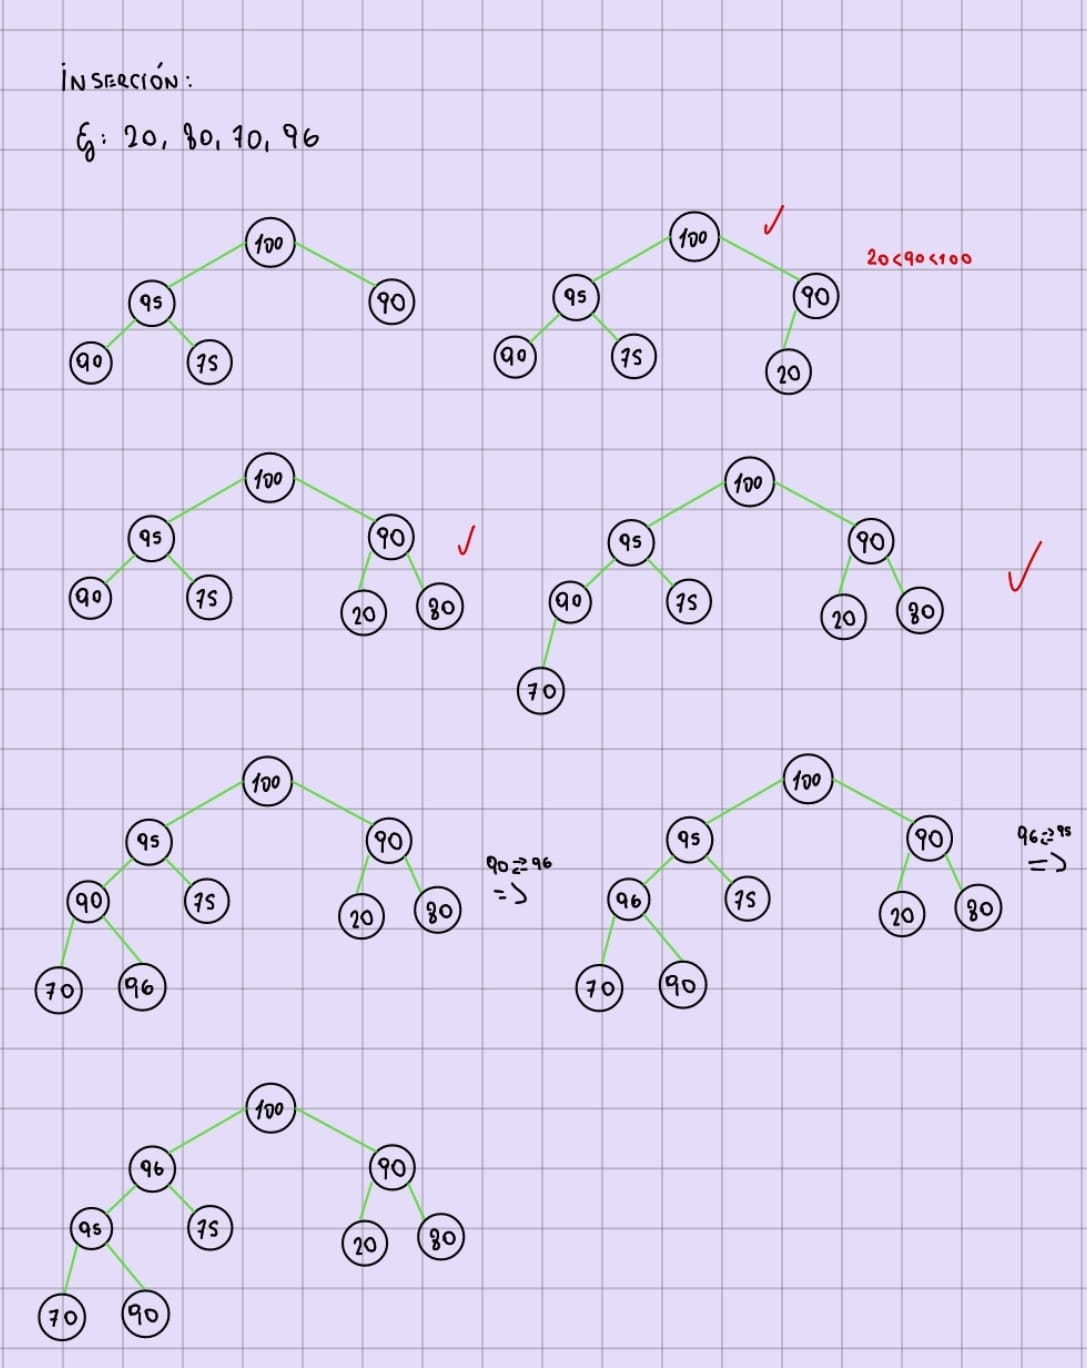
\includegraphics[width=\linewidth]{assets/insertando_heaps.jpg}
        \centering
        \label{fig:insertando_en_heaps}
    \end{minipage}
\end{center}
\textbf{Desencolar / Borrar}:
\begin{center}
    \begin{minipage}[b]{0.5\textwidth}
        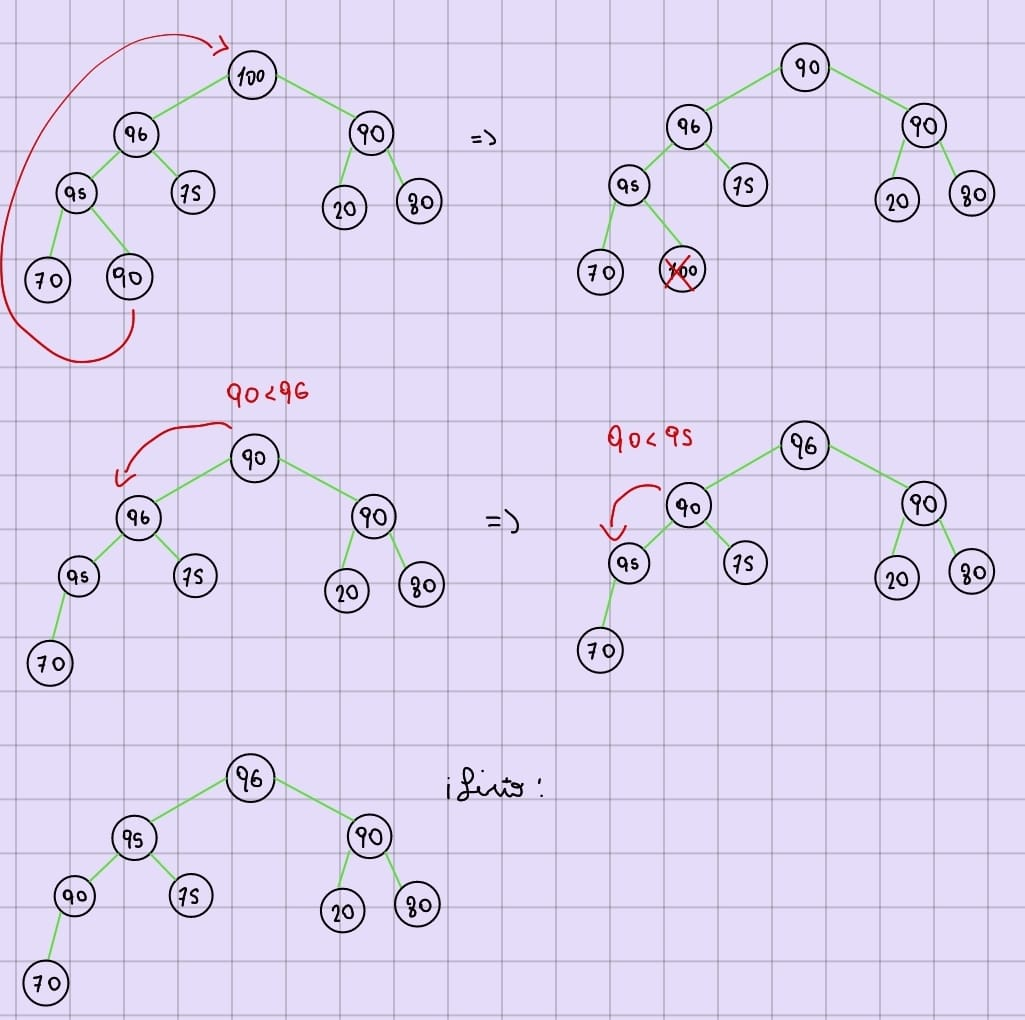
\includegraphics[width=\linewidth]{assets/borrar_heaps.jpg}
        \centering
        \label{fig:borrar_heaps}
    \end{minipage}
\end{center}
Nota: Nótese que es importante si está implementando un max-heap o un min-heap, porque en el max-heap tenemos que reacomodar de manera que quede en la raíz el más grande mientras que en el min-heap tenemos que dejar el más chico.
\subsection*{Implementacion de Heaps de maneras diversas}
\label{subsec:implementaciones_heap}
\textbf{Sobre Array}
Sabemos que un Heap es lo más cercano a ser implementado con árboles binarios balanceados. \\ 
Consideremos que debemos implementarlo con un array ¿como lo haríamos? \\
La manera de representarlo en un array es: raiz - hijo izq - hijo der - hijo izq de hijo izq, hijo der de hijo izq - hijo izq de hijo der, hijo der de hijo der. \\
Es como que vas tomando misma altura, pero completas primero con izquierda y luego derecha. \\
Fórmula (invariante): 
\begin{itemize}
    \item si v es la raiz, entonces v es el primero del arreglo.
    \item si v es el hijo izquierdo de u entonces 2p(u)+1
    \item si v es el hijo derecho de u entonces 2p(u)+2
\end{itemize}
\begin{center}
    \begin{minipage}[b]{0.6\textwidth}
        \includegraphics[width=\linewidth]{assets/heap.png}
        \centering
        \label{fig:heap}
    \end{minipage}
\end{center}
Transformado a array sería: $[89, 67, 68, 66, 65, 66, 67, 1, 43, 21, 5, 4, 64]$ \\
Ventajas de implementar Heap con Array: 
\begin{itemize}
    \item Ventajas:
    \begin{itemize}
        \item Muy eficiente en términos de espacio.
        \item Es fácil de navegar.
    \end{itemize}
    \item Desventajas:
    \begin{itemize}
        \item Al ser un arreglo, es necesario duplicar el arreglo o achicarlo a medida que se agregan o eliminan elementos.
    \end{itemize}
\end{itemize}
\subsection*{Array $\rightarrow$ Heap (Array2Heap)}
\label{subsec:array_2_heap}
\begin{itemize}
    \item Forma 1 (Costo $\theta(n \ log(n))$): Permutando sus elementos, hasta llevarlo a un heap y que cumpla el invariante de representación. Si no recuerda qué reglas debe cumplir el array, véase \hyperref[subsec:implementaciones_heap]{\underline{implementaciones heap}}.
    \item Forma 2 (Costo $\theta(n)$), Algoritmo de Floyd: Estrategia bottom-up. Desde el último sub-heap de la derecha, voy viendo si cada uno son un heap válido, si no lo son aplico la operación bajar en el elemento padre de ese sub-heap. Si ya llegué al último sub-heap de la izquierda, vuelvo a la derecha pero voy al padre del último padre de la derecha.
\end{itemize}

\end{document} 
